\chapter{\texorpdfstring{\acrlong*{acc:ea}}{Evolutionary algorithms}}
\label{chap:eva}

Optimization. What better word would describe the ultimate goal of all the people, our civilization, and maybe even the Universe. With a bit of exaggeration, optimization is the cause of all the ramifications we can see around. What else are physics laws than minimization processes, our pursuit of knowledge and self--improvement rather than maximization of self-worth, industrial revolutions than minimization of human labor, maximization of goods production, and standard of living at the same time. In my opinion, optimization is the reason what drives us forward, makes us better, and guides our decisions.

One of the most extraordinary optimization processes is, without a doubt, evolution. Evolution is nothing less than Nature's way of improving species to better adapt to their environment. The father of evolution is undoubtedly Charles, who first come up with an idea of evolution in his work \enquote{On the origin of species: A facsimile of the first edition} \citep{darwin1964origin}. According to him, the individuals better adapted to the environment have a higher potential to reproduce and pass their genetic material --- including the predisposition to survive in the environment --- to their offsprings. Sometimes referred to as \enquote{Survival of the fittest}.

This exact ideas inspired scientists and formed the field of \acrfull{acc:ea}\index{evolutionary algorithm}\footnote{I will refer to all the population-based algorithms in this work as \acrlong*{acc:ea}. These includes, among others, \acrlong*{acc:ga}, \acrlong*{acc:es}, and \acrlong*{acc:pso}.}.
\acrshort{acc:ea} are stochastic, population-based optimization algorithms inspired by biological evolution. In general, a set of individuals called the population compete with each other for a place in the next generation. Each individual represents one possible solution to the problem at hand. The quality of the individual is proportional to the quality of solution it represents. This quality is usually expressed using the fitness (or sometimes called objective) function. As with natural evolution, the probability of survival is proportional to the solution quality -- the better the solution is, the higher the probability of survival \citep{IntroductionToEA}. In the \acrshort{acc:ea}, the process producing new generation is usually called selection.

Evolution is not only about survival but also about reproduction. \acrlong*{acc:ea} took inspiration here as well and uses specials operators for each generation -- usually called evolution operators or variation operators\index{variation operator}. As the name suggests, these operators make sure the population explores new solutions. The two most common operators are crossover and mutation. During crossover\index{crossover}, individuals from the current population (usually called parents) produce new individuals (usually called offsprings) by combining their genetic information. In some way, crossover mimics reproduction in Nature, during which the \acrshort{acc:dna} of offspring is by majority determined by its parents \acrshort{acc:dna}. Mutation\index{mutation}, on the other hand, causes random minor alteration of the individual genetic material and is able to introduce novel patterns that did not previously occur in the population \citep{HowToSolveItModernHeuristics}.

In general, \acrshort{acc:ea} repeat steps above until a sufficiently good solution is found or until a maximum number of generations is reached. The general pseudocode of the \acrshort{acc:ea} algorithm is in Algorithm \ref{alg:SEA}. I will present more accurate implementations of various algorithms through this chapter.

\begin{algorithm}
    \SetAlgoLined
    \KwResult{evolved population}
    initialize population\;
    \Repeat{termination criteria met}{
        reproduction\;
        mutation\;
        evaluate population\;
        selection\;
    }
    \caption{General Evolution Algorithm}
    \label{alg:SEA}
\end{algorithm}




%%%%%%%%%%%%%%%%%%%
%%               %%
%%  TERMINOLOGY  %%
%%               %%
%%%%%%%%%%%%%%%%%%%
\section{Terminology}

This section will introduce the necessary terminology that I am going to use throughout this work. I took most of the terminology from \citet{IntroductionToEA}.

\defterm{Problem} is the function we want to solve. It can be both a satisfactory as well optimization problem.

\defterm{Genotype}\index{genotype} is encoding of the solution. It is equivalent of the \acrshort{acc:dna} -- it compress all the data needed to produce solution.

\defterm{Gene} is one part of the genotype. It may be one bit if the genotype is encoded as a binary string or scalar if the genotype is a vector. 

\defterm{Representation or genotype space} is the space of genotype.

\defterm{Phenotype}\index{phenotype} is the solution built from genotype. Genotype and phenotype can be equivalent -- for example, a real function optimization problem may have a genotype vector of real numbers representing one of the solutions. Generally, however, genotype and phenotype can be different \citep{GeneticAlgorithmEssentials}.

\defterm{Search space} is the space of phenotype.

\defterm{Objective function} is the function the algorithm optimize. For the previous example of real function optimization, the function itself can be the objective function. I will denote objective function $\objectivefn$.

\defterm{Fitness function}\index{fitness function} is the measure of the quality of the solution. Note that the domain of the function is the search space. Unlike the objective function, the fitness function should guide the algorithm during the optimization. It can use the objective function directly, but other options are possible as well. For example, if the goal is to maximize objective function $\objectivefn(x)$, but the algorithm is written such that it minimize the fitness function, one may specify the fitness function as $\fitnessfn(x)=\frac{1}{\objectivefn(x)}$. I will denote fitness function $\fitnessfn$.

\defterm{Evaluation} is the process of obtaining fitness value for the genotype.

\defterm{Individual} is a genotype with its fitness value. I will denote individual by $\individual$.

\defterm{Fitness value} of the individual is its evaluation. 

\defterm{Population} is a multiset of individuals -- it is possible to have the identical genotype in the population multiple time. However, I will still distinguish different individuals with the same genotype. I will denote the whole population as $\population$.

\defterm{Initialization} is the process of creating the first population.

\defterm{Exploitation} is the effort to use knowledge from the history in order to maximize the expected outcome \citep{SelfAdaptiveFeaturesInRealParameterEvolutionaryAlgorithms}.

\defterm{Exploration} is the effort to discover new rules about the problem at hand, although the expected outcome does not need to be the best possible. In general, the biggest problem in \acrshort{acc:ea} is the right balance between exploitation and exploration. Putting too much emphasis may cause getting stuck in the local minima, whereas putting too much focus on the exploration may cause the algorithm never to converge. Note that \acrshort{acc:ea} is not the only field suffering from this, but for example Reinforcement Learning deals with the same problems \citep{ExplorationExploitationDilemaRL}. 

\defterm{Evolution operators} are individual steps performed each iteration.

\defterm{Selection}\index{selection} is an evolution operator that draws individuals from the current population to the next one. The selection should consider the fitness value of each individual in the population and pick them proportionally. Selection, therefore, implements the \enquote{Survival of the fittest} law. From the mathematical point of view, selection task is to move the population into the more promising area of the search space and possibly to reduce the variance of the population \citep{SelfAdaptiveFeaturesInRealParameterEvolutionaryAlgorithms}. In other words, selection is the exploitation step in the algorithm.

\defterm{Crossover}\index{crossover} is evolution operator, that combines some individuals (usually called \textbf{parents}) in order to create one or more new individuals (usually called \textbf{offsprings}). Offsprings are usually combination of their parents, similarly to how \acrshort{acc:dna} of the child is combination of \acrshort{acc:dna} of her parents.

\defterm{Mutation}\index{mutation} is evolution operator, that modify one individual. Mutation can be based on randomness (for example replacement of value in genotype by different value) or specialized for the problem in hand. This time the example can be \acrlong{acc:tsp}, where one possible mutation operator can \enquote{untwist} ways that cross each other. This mutation is, in fact, a local optimization technique, as the mutated way is shorter than the previous one \citep{TSPArticle}.

\defterm{Variation operators}\index{variation operator} are operators that change the variation of the population, but not the mean. Variation operators are the exploration steps in the algorithm and should balance the exploitation strength of the selection. Both crossover and mutation are variation operators \citep{SelfAdaptiveFeaturesInRealParameterEvolutionaryAlgorithms}.

\defterm{Memetic operator} is an operator that uses local optimization in every iteration. Alternatively, \enquote{memetic algorithms uses local optimizer to every solution before evaluation} \citep{HowToSolveItModernHeuristics}. One such example is the mutation operator for \acrlong{acc:tsp} problem mentioned earlier. Another example is the training of \acrshort{acc:ann}. The memetic operator would be one run of the backpropagation algorithm in each generation.




%%%%%%%%%%%%%%%%%%%%%%%%%%
%%                      %%
%%  GENETIC ALGORITHMS  %%
%%                      %%
%%%%%%%%%%%%%%%%%%%%%%%%%%
\section{\texorpdfstring{\acrlong*{acc:ga}}{Genetic algorithms}}

\acrfull{acc:ga}\index{genetic algorithm} are probably the simplest \acrfull{acc:ea} out there and as their father is usually considered \citefullauthor{HollandGA}. In the \acrshort{acc:ga}, individual are binary string of length $n$, formally
$$ \individual \in \left\{0,1\right\}^{n} $$

Fitness function maps genotype into real values
$$ \fitnessfn:\left\{0,1\right\}^{n}\rightarrow\mathbb{R} $$

The typical crossover operator is \emph{one point crossover}\index{crossover \acrshort*{acc:ga}!one--point}. This type of crossover requires two parents and produces two offsprings. As the first step, the algorithm uniformly sample random integer $s$ in the range $\left[ 1, n-1 \right]$. The first offspring will receive genetic material up to index $s$ from the first parent and the rest from the second one. The second offspring is created the same way, except the position of parents is exchanged. Example for $n=10$ is in figure \ref{fig:gaonepointcrossover}. In order not to modify all the individuals in the population, only $p_c\in\left[0,1\right]$ percent of individuals undergo the crossover, and the children replace their parents \citep{IntroductionToEA}.

\begin{figure}
    \begin{subfigure}[b]{0.4\textwidth}
        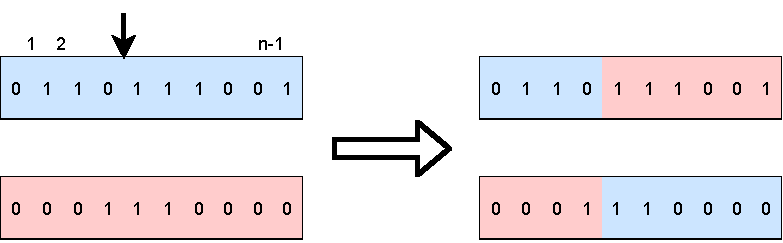
\includegraphics[width=\textwidth]{img/master_onepointcrossover.pdf}
        \caption{One point crossover}
        \label{fig:gaonepointcrossover}
    \end{subfigure}
    \hfill
    \begin{subfigure}[b]{0.4\textwidth}
        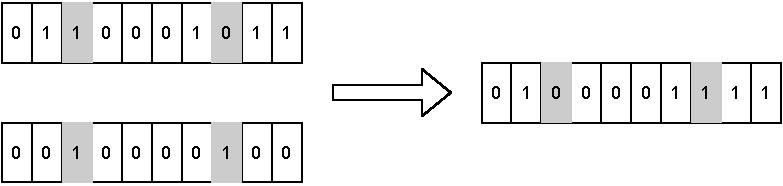
\includegraphics[width=\textwidth]{img/master_bitflipmutation.pdf}
        \caption{Bit--flip mutation}
        \label{fig:bitflipmutation}
    \end{subfigure}
    \caption{Genetic algorithm operators}
\end{figure}

The mutation\index{mutation \acrshort*{acc:ga}} operator for \acrshort{acc:ga} is in the most cases bit--flip mutation\index{mutation \acrshort*{acc:ga}!bit--flip}. During this mutation, each gene in the genotype mutates with probability $p_m$. One example of mutation is in figure \ref{fig:bitflipmutation}. Mutation has two objectives -- it makes sure the algorithm is not trapped in local optima and sustains genetic disparity in the population. As a side effect, mutation serves as a secondary search operator \citep{IntroToGA}.

The difference between crossover and mutation is such that crossover is rather \enquote{search} exploitation technique. It combines individuals from the current population and exploits them to find possibly better individuals. On the other hand, the mutation is a more local search technique, and based on the probability $p_b$, it searches over the whole representation space.

Finally, the selection stage takes place. There are various selection techniques, and in this particular case, I will use tournament selection\index{selection!tournament}. Tournament selection compares two random individuals' fitness values and places the better individual is into the new population. This repeats as many times as needed to form a new population.

For cases where the population's size does not change between generations, there is a high probability that the same individual will be in the following population multiple times. Nonetheless, because variation operators (crossover and mutation) keep divergence in the population, duplicities in the population are not a problem.

The pseudocode of the simple genetic algorithm described above is depicted in algorithm \ref{alg:SGA}. Firstly, the population is randomly initialized and then undergo crossover, mutation, evaluation, and selection operators in the loop. Finally, the evolved population is returned from the algorithm.

\begin{algorithm}
    \KwIn{$d$ problem dimension, $l$ population size, $g$ generations, $\fitnessfn$, $p_c$, $p_m$}
    \KwResult{evolved population}
    population $\leftarrow$ randomly initialized\;
    \ForEach{$gen$ in $0$..$g$}{
        \ForEach{individual in $0$..$l$}{
            \If(){$rand()<p_c$}{One point crossover with random individual}
            \If(){$rand()<p_m$}{Bit--flip mutation}
        }
        Evaluate population using $\fitnessfn$\;
        population $\leftarrow$ pick up $l$ individuals using tournament\;
    }
    \Return{population}
    \caption{Simple genetic algorithm}
    \label{alg:SGA}
\end{algorithm}

I will refer to the algorithm described above as \enquote{Simple Genetic Algorithm}. In reality, scientists come up with various operators that can improve convergence or can help in specific types of problems. Through the following paragraphs, I will focus on these techniques, inspired mainly by the book of authors \citet*{IntroToGA}.

%%%%%%%%%%%%%%%%%%%%%%
%%%%  CROSSOVERS  %%%%
%%%%%%%%%%%%%%%%%%%%%%
\subsection{Advanced crossover operators}

The simple genetic algorithm used one point crossover. It is straightforward to extend it into \emph{two points crossover}\index{crossover \acrshort*{acc:ga}!two points} where each genome is split into three parts. Each offspring then receives first and third part of the genome from one parent and the middle one from the second one. An example of two points crossover is in the picture \ref{fig:gatwopointcrossover}.

\begin{figure}
    \begin{subfigure}[b]{0.4\textwidth}
        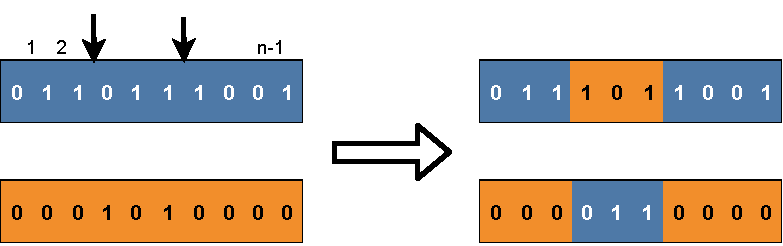
\includegraphics[width=\textwidth]{img/master_twopointcrossover.pdf}
        \caption{Two point crossover}
        \label{fig:gatwopointcrossover}
    \end{subfigure}
    \hfill
    \begin{subfigure}[b]{0.4\textwidth}
        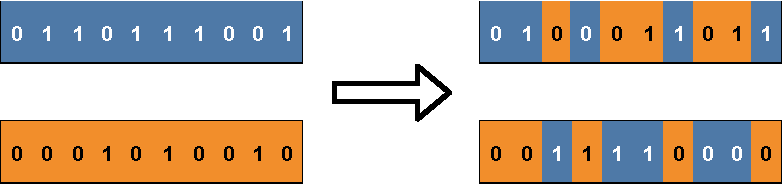
\includegraphics[width=\textwidth]{img/master_uniformcrossover.pdf}
        \caption{Uniform crossover}
        \label{fig:uniformcrossover}
    \end{subfigure}
    \caption{Advanced crossover operators}
\end{figure}

Sometimes, the crossover operator is generalized even more and forms $k$--point crossover. The genotype partitions into $k$ parts, and these parts are interleaved in the offsprings. A special case is \emph{uniform crossover}\index{crossover \acrshort*{acc:ga}!uniform} -- the offsprings are constructed in such a way that they are a uniform combination of their parents. Each gene in the offspring has an equal probability of whether it will be received from the first or second parent. The second offspring will follow the same pattern, except with parents swapped. Example of uniform crossover is in figure \ref{fig:uniformcrossover}.
% Introduction into GA presents few more types - three parents crossover, crossover with a reduced surrogate, and shuffle crossover. These are irrelevant for my implementation, but I can potentially describe them here.

I have described the crossover operators such that the offsprings replace their parents. That is a popular design decision, however, one does not need to enforce it and may decide to create offsprings in addition to the parents. To ensure the population does not increase in size over the generations, the selection operator can be implemented in a way that a specified number of individuals will be drawn up.

%%%%%%%%%%%%%%%%%%%%%
%%%%  SELECTION  %%%%
%%%%%%%%%%%%%%%%%%%%%
\subsection{Selection operators}

The selection operator is one of the most important ones. It is the only operator working with fitness values; therefore, the operator is responsible for exploitation in the algorithm. The simple genetic algorithm presented in algorithm \ref{alg:SGA} uses tournament selection -- I will analyze other types of selections through the following paragraphs.

Selection operators are equivalent to Darwin's selection process in Nature. It allows to preserve perspective genetic traits and discard the bad ones. That answer to the \enquote{Survival of the fittest} idea. The distinction between good and bad individuals is in respect to the fitness function; selection operators, therefore, favor individuals with better fitness value.

The degree into which operators endorse better individuals is called \emph{selection pressure}\index{selection pressure}. Selection pressure is a primary indicator of the algorithm and needs to be balanced with other variation operators. Too immense selection pressure may cause the algorithm to converge prematurely. On the other hand, too weak selection pressure may prolong the convergence, and the algorithm may need unnecessary steps before convergence.

\emph{Tournament selection}\index{selection!tournament} is one of the most popular selection operators because it is easy to implement, and the absolute values of fitness are not relevant (rather relative difference to the other individuals is what matter). Tournament selection, therefore, keeps the selection pressure constant. Tournament selection can be naturally extend using $k$ parents -- it increases the probability for better individuals and thus increases the operator's selection pressure.

Another popular operator is \emph{Roulette Wheel selection}\index{selection!roulette}. In this operator, the probability of selection is equal to the absolute value of the fitness.
$$ P\left[\individual_i\right] = \frac{\fitnessfn(\individual_i)}{\sum_{j=0}^{l}\fitnessfn(\individual_j)} $$
This can be imagined as a roulette wheel, where individuals represent a sector of a wheel. The size of the sector is proportional to the fitness value of the individual. The selection procedure to pick up $n$ individuals simply spins the roulette $n$--times and selects the individual on which the roulette stopped. An example of roulette wheel selection is in figure \ref{fig:roulettewheelselection}. Selection operators that depend on the absolute values of fitness value are usually called proportional--based selection\index{selection!proportional--based}.

Slight improvement of roulette wheel selection is \emph{Stochastic Universal Sampling}\index{selection!stochastic universal sampling}. Because roulette wheel selection samples individuals independently, it may select the same individuals more time than would be expected given its proportion to the rest of the population. In the example in figure \ref{fig:roulettewheelselection}, the expected number of draws for individual $p_3$ is one. However, it has been drawn two times. Stochastic Universal Sampling handles this issue by sampling only one number in the range $\left[0,\frac{\sum_i^l\fitnessfn(p_i)}{l} \right]$ and draw each new individual with $\frac{\sum_i^l\fitnessfn(p_i)}{l}$ offset. The stochastic universal sampling is unbiased, and the distribution of drawn individuals is closer to the fitness values distribution in contrast to the roulette wheel selection. An example of stochastic universal sampling is in figure \ref{fig:USB}.

\begin{figure}
    \begin{subfigure}[t]{0.47\textwidth}
        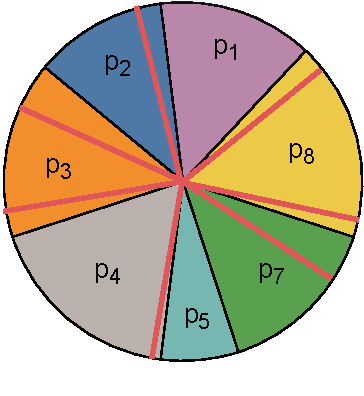
\includegraphics[width=0.8\textwidth]{img/master_roulettewheel.pdf}
        \caption{Roulette wheel selection. Red lines represents sampled individuals.}
        \label{fig:roulettewheelselection}
    \end{subfigure}
    \hfill
    \begin{subfigure}[t]{0.47\textwidth}
        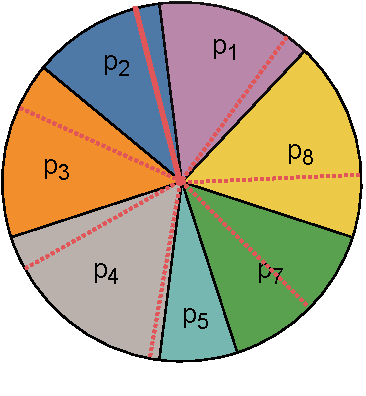
\includegraphics[width=0.8\textwidth]{img/master_stochasticuniversalsampling.pdf}
        \caption{Stochastic universal sampling. Red line represent sampled number and dotted lines are sampled individuals with $\frac{1}{7}$ offset.}
        \label{fig:USB}
    \end{subfigure}
    \caption{Roulette based selections}
\end{figure}

Notice that for both selection operators, individuals with the higher fitness value have a higher probability of being picked up to the successive population. These operators are therefore intended for maximization problems. Also, because the fitness value directly affects the circle sector's size, the fitness function must be positive over the whole domain. It is possible to discard individuals with non--positive fitness values; however, then the whole selection procedure would lose relevance.

One more drawback of both roulette wheel selection and stochastic universal sampling is that the probabilities depend on fitness's absolute values. Let us look at two cases:
\begin{itemize}
    \item The population fitness values are distributed in the range $\left[ 99,100 \right]]$.
    \item The population fitness values are distributed in the range $\left[ 1, 2\right]$.
\end{itemize}
In both cases, the expected difference of fitness between any two individuals is the same. Nevertheless, because roulette wheel selection takes into account absolute values of fitness, the probability of drawing the best individual from the first case is much smaller compared to the second case. This is a side effect of proportional--based selection.

The drawback of proportional--based selection is that it does not create enough selection pressure when the population has roughly the same fitness value. This problem occurs at the end of the evolution because all the individuals are optimized over the generations and usually have very similar fitness values. Note that tournament selection does not suffer from this, as only the relative order between individuals determines the selection order.

One way to eliminate this problem is to rescale fitness to have more desired properties\index{fitness scaling}. One common example is linear scaling into interval $\left[ l,u \right]$ so that individual with $\min\fitnessfn(x_i)=l; \max\fitnessfn(x_i)=u$ and rest of them is scaled linearly between them. 
$$
f_{scale}(\individual)=\frac{\fitnessfn(\individual) - \min\limits_{i}\fitnessfn(\individual_i)}{\max\limits_{i}\fitnessfn(\individual_i)}\cdot(u-l)+l 
$$
Alternatively, logarithmic respectively exponential scale is possible as well, so there will be more emphasis on individuals from the beginning of the sorted sequence, respectively lesser importance of individuals from the end.

Special example of fitness scaling is \emph{rank selection}\index{selection!rank}. To eliminate dependency on the fitness function's absolute values, rank selection assigns artificial fitness values to the individuals based on their order in the sorted sequence. One common rank evaluation function is linear -- it assigns new fitness values in the interval $\left[l,u\right]$ such that the best individual has new fitness value $l$, the worst one $u$, and the rest of the population is uniformly distributed in this interval \citep{razali2011genetic} (I expect minimization problem). Different scaling schemas are possible as well.

The advantage of rank selection is steady selection pressure, and unlike mentioned roulette wheel selection, it can handle fitness functions with negative values. Moreover, it is easy to control selection pressure using interval width, as shown in table \ref{tab:rankselection}. It also does not suffer from outliers -- individuals with very high or low fitness in comparison to the rest of the population. Rank selection can avoid premature convergence, but computation costs can be very costly because the population needs to be sorted, fitness values reevaluated, and another proportional--based selection operator needs to follow.

\begin{table}
    \centering
    \begin{tabular}{|c c | c c | c c |}
        \hline
        \thead{Fitness\\value} & Rank & 
        \thead{New fitness\\for $\left[1,2\right]$}  & 
        \thead{Selection\\probability\\for $\left[1,2\right]$} &
        \thead{New fitness\\for $\left[1,10\right]$} &
        \thead{Selection\\probability\\for $\left[1,10\right]$} \\
        \hline
        12   & 1   & 2     & $27\%$ & 10    & $38\%$ \\
        7    & 2   & 1.75  & $23\%$ & 7.5   & $29\%$ \\
        1    & 3   & 1.5   & $20\%$ & 5     & $19\%$ \\
        0    & 4   & 1.25  & $17\%$ & 2.5   & $10\%$ \\
        -5   & 5   & 2     & $13\%$ & 1     & $4\%$  \\
        \hline
    \end{tabular}
    \caption{Rank selection pressure}
    \label{tab:rankselection}
\end{table}

Selection operators may use traditional approaches from search algorithms -- for example \emph{simulated annealing}\index{selection!simulated annealing}. Simulated annealing is an analogy to metallurgy, whereby precise control of heating and cooling of material is improved its physical and chemical properties. In general, it accepts worse solutions as long as the temperature $\tau$ is high enough. The temperature $\tau$ starts high, so almost all the solutions are accepted from the beginning. The temperature slowly decreases during a run of the algorithm down to the value zero. Decrease is usually exponential: $\tau_g=\tau_0(1-\alpha)^{1+\frac{\beta\cdot g}{G}}$ where $g$ is current generation, $G$ maximum number of generations, $\alpha\in\left[0,1\right]$, $\beta\in\mathbb{R}^+$, and $\tau_0\in\mathbb{R}^+$ are parameters. 

One example of simulated annealing is the Boltzmann selection operator. It draws the individuals with probability 
$P=exp\left(-\frac{f_{max} - \fitnessfn(\individual)}{\tau}\right)$
where $f_{max}$ is the best fitness in the population and $\tau$ is the current temperature (known as Boltzmann probability). Note that Boltzmann selection is once again proportional--based selection operator and may suffer from the same problems as roulette wheel selection.
% TODO Boltzmann selection not implemented

The last selection operator, I would like to discuss, is \emph{elitism}\index{elitism}. For some problems may be beneficial to preserve the best individuals from the population. This is especially helpful for problems where the algorithm can find the optimal solution using small local steps. Mutation and crossover may destroy the best individual in the population, and it may be difficult for the algorithm to found it once again if its genetic material has not been propagated yet.

The elitism mechanism is operator, which makes sure the best individuals endure in the population. It is usually implemented in a way it copies the $k$ best individuals from the population before all other operators execute, and copy them back afterward. Note that elitism is not truly a selection operator, but rather an insure mechanism not to lose the population's best individuals. Traditional selection operator still needs to be present in order for the algorithm to work. 

% TODO I did not discuss the schemata; it may be worth mentioning them




%%%%%%%%%%%%%%%%%%%%%%%%%%%%%
%%                         %%
%%  REAL CODED ALGORITHMS  %%
%%                         %%
%%%%%%%%%%%%%%%%%%%%%%%%%%%%%
\section{Real--Coded Evolutionary Algorithms}

Real--coded evolutionary algorithms are natural extension of \acrshort{acc:ga} by extension of genotype into real numbers.
$$
\individual \in \mathbb{R}^{n}
$$
Alternatively, the relaxed definition allows genotype of an arbitrary number of dimensions. That may be helpful for problems, which expect a particular structure of the solution -- for example image processing filters \citep{WVDF}. Note that using the different genotype structure disallows direct use of some operators, like one and two--point crossovers, because the split point may be ambitious. On the other hand, some operators, like the uniform crossover, can easily handle multidimensional genotypes without much change.

Origin of real--coded evolutionary algorithms, more precisely \acrfull{acc:es}, dates back to 1970s at Technical University in Technische Universität Berlin, where \citeauthor*{ES-original} presented \acrshort{acc:es} \citep{ES-original}. Originally, \acrshort{acc:es} has not been used as an optimization algorithm for real function, but \enquote{rather as a set of rules for the automatic design and analysis of consecutive experiments with stepwise variable adjustement driving a suitable object/system into the optimal state in spite of environmental noise} \citep{EScomprehensiveintroduction}. It turned out that this simple stochastic search technique outperformed traditional--based methods. Although there is no guarantee \acrshort{acc:es} will find the optimal solution, they are in most cases able to find near--optimal and sufficiently good enough solution.

This section takes inspiration mainly from the work of \citet*{IntroductionToEA} and \citet*{EScomprehensiveintroduction}. Moreover, some techniques originated in \acrshort{acc:es} are applicable for general real--coded evolutionary algorithms as well. Therefore, I will not make rigorous distinction between real--coded evolutionary algorithms and \acrshort{acc:es} through this section.

Real--coded evolutionary algorithms can use same selection and crossover operators as \acrshort{acc:ga}, although it is not recommended \citet{IntroductionToEA}. In general, good crossover operators should
\begin{itemize}
    \item preserve population mean because crossover operators do not work with a fitness function and therefore should introduce bias in the search space,
    \item slightly increase the variance of the population, to balance the pressure of selection operators, that usually decrease the variance of the population,
    \item\label{enum:espopulationvariance} \snipescondition, so the algorithm effectively search neighborhood solutions,
    \item allows reachability of any solution in the search space.
\end{itemize}
Crossover operators from \acrshort{acc:ga} may fulfill these requirements, however, real--coded encoding allows a more diverse set of operators. I will describe them a bit later.

\acrshort{acc:es} also introduced two different selection schemas\index{selection schema}:
\begin{itemize}
    \item $\left(\mu+\lambda\right)$ evolution strategy, also known as \emph{plus schema}.
    \item  $\left(\mu,\lambda\right)$ evolution strategy, also known as \emph{comma schema},
    \item\label{enum:steadystate} steady--state evolution strategy.
\end{itemize}
Here, the $\mu$ represents a number of parents and $\lambda$ number of offsprings. In the first two cases, $\abs{\mu}$ individuals are picked to the next generation. In the plus schema, these individuals are taken from both parents and offsprings. For the comma schema, $\abs{\mu}$ individuals are drawn only from the offsprings, and parents are discarded. Obviously, to have at least $\abs{\mu}$ distinct individuals in the next generation, it must hold $\lambda\geq\mu$. For stochastic selection operators, where is the possibility to draw the same individual multiple times, it may be beneficial to have more offsprings than parents.

Both plus and comma selection schemas generate $\mu$ offsprings and resample the whole population for the next generation. Steady--state evolution strategy, on the other hand, generates just one (or a very few) individuals in each generation and tries to reintegrate them back into the population. The steps of the algorithm are:
\begin{enumerate}
    \item Generate a new individual and evaluate it using the fitness function.
    \item\label{enum:steadystateparentpickup} Choose an individual from the population that the new one can replace.
    \item\label{enum:steadystatereplacement} Decide whether the new individual should replace the old one.
\end{enumerate}
The step \ref{enum:steadystateparentpickup} is known as the replacement strategy, and some of the common variants are to replace the oldest, worst, or random individual. The step \ref{enum:steadystatereplacement} is known as the replacement condition. The most common variant is to replace the old individual only if the new one is better; however, it is as well possible to use simulated annealing.
The steady--state expresses the idea that the population undergoes only a tiny change in each generation \citep{SteadyStateEvolutionStrategy}.

%%%%%%%%%%%%%%%%%%%%%%
%%%%  CROSSOVERS  %%%%
%%%%%%%%%%%%%%%%%%%%%%
\subsection{\texorpdfstring{\acrshort*{acc:ea} crossovers}{Crossovers}}

Encoding genotype as a vector of real numbers allows, except crossover operators from \acrshort{acc:ga}, additional crossover operators using real numbers. One argument may be to exploit correlation within the population.

\begin{figure}
    \begin{subfigure}[t]{0.49\textwidth}
        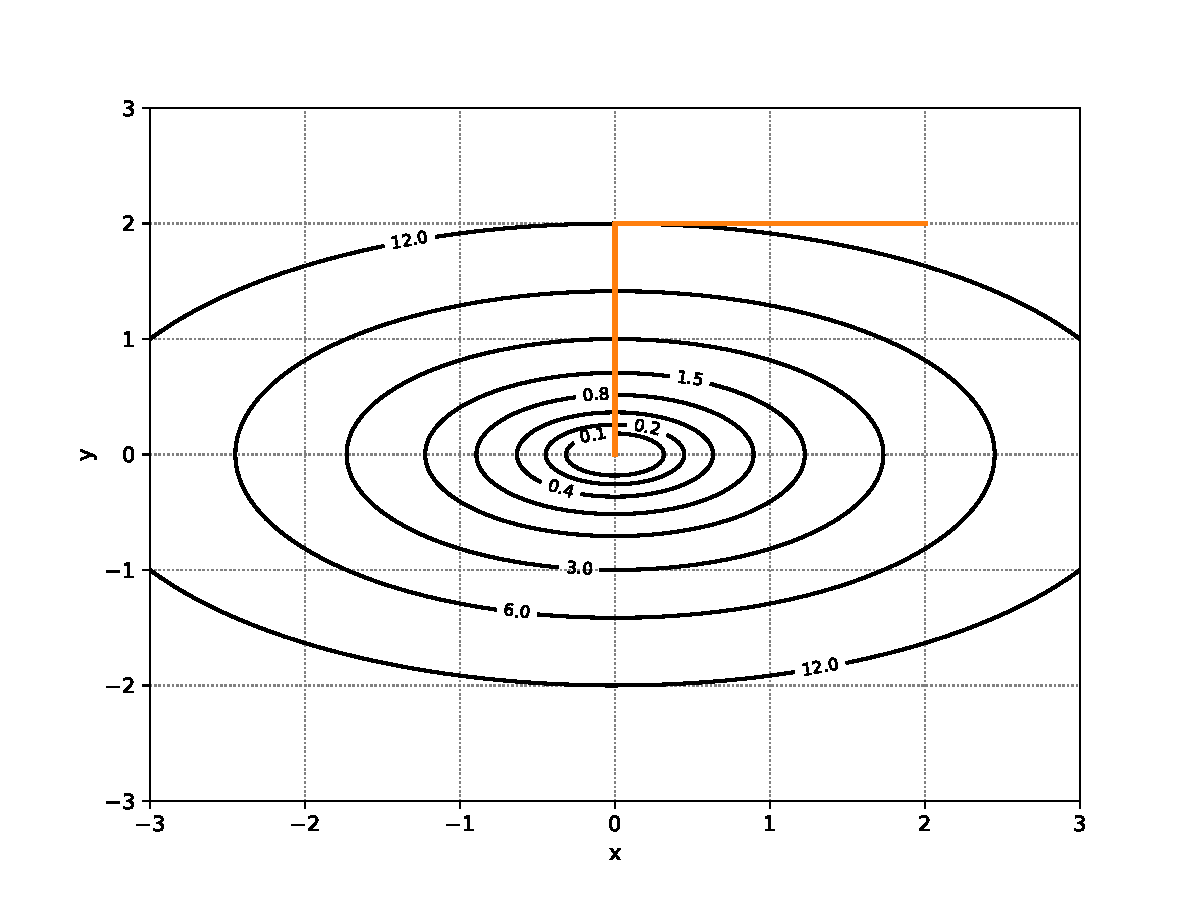
\includegraphics[width=\textwidth]{img/render_separable.pdf}
        \caption{Separable ellipsoid function.}
        \label{fig:separableelipsoid}
    \end{subfigure}
    \hfill
    \begin{subfigure}[t]{0.49\textwidth}
        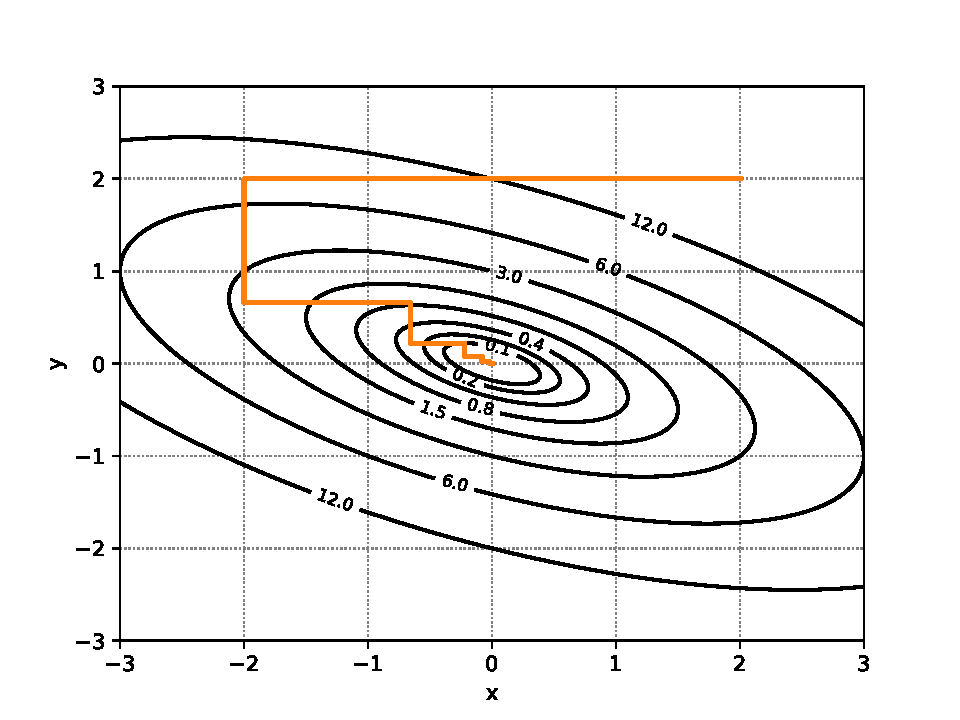
\includegraphics[width=\textwidth]{img/render_nonseparable.pdf}
        \caption{Non--separable ellipsoid function.}
        \label{fig:nonseparableelipsoid}
    \end{subfigure}
    \caption[Difference between separable and non--separable function for optimization]{Difference between separable and non--separable function for optimization. Trajectories of hill climbing algorithm are depict orange.}
    \label{fig:separationfucntions}
\end{figure}

Lets take for example two functions:
\begin{align*}
    f_{sep}(x,y)&=x^2+3y^2 \\
    f_{nosep}(x,y)&=x^2+3y^2+2xy
\end{align*}
These functions are shown in figure \ref{fig:separationfucntions}. Running simple hill climber algorithm \citep{HandbookOfMetaheuristics}, one may get trajectories displayed in the figure by orange color. Notice that the trajectory of the function $f_{nosep}$ is much longer -- it took $200$ steps to achieve global minimum for the function $f_{sep}$, however up to $400$ steps for the function $f_{nosep}$ (the step size was equal for both runs). The cause of this is that the first function is separable -- it can be written in the form $f_{sep}(x,y)=f(x)+f(y)$. Hill climbing algorithm can easily find optimum because $\min f_{sep}=\min f(x)+\min f(y)$, therefore it can search for the optimum for each variable and then aggregate the outcomes. That is not true for the function $f_{nosep}$, because it is not separable, and using the local search technique is not as straightforward. Separable functions are more challenging and harder in some sense, exactly the kind of problems \acrshort{acc:ea} should solve efficiently.

The problem of crossover operators from \acrshort{acc:ga} is precisely the same as I have just shown you. These operators work on the genes independently and do not use knowledge about the correlation of the genotype space within the population. It is necessary to use different crossover operators tailored for the real--coded \acrshort{acc:ea}.

One of the simplest real--coded \acrshort{acc:ea} crossover is \emph{arithmetic crossover}\index{crossover real--coded!arithmetic}. For parents $\mathbf{p_1}$ and $\mathbf{p_2}$, the offspring $o$ is created using following formula.
$$
\mathbf{o} = \alpha\mathbf{p_1}+\left(1-\alpha\right)\mathbf{p_2}
$$
where $\alpha \sim U(0,1)$ (uniformly distributed variable in interval $\left[0,1\right]$). Is is possible to generate second offspring by setting $\beta=1-\alpha$ and substitute $\beta$ for $\alpha$. This operator uses same $\alpha$ for every dimension of the vector, so it is sometimes called \emph{whole arithmetic crossover}. Easy extension is to use $\boldsymbol{\alpha}=(\alpha_1,\alpha_2,\dots,\alpha_n)$ vector, where $\alpha_i\sim U(0,1)$ and create offspring using similar formula.
$$
\mathbf{o} = \boldsymbol{\alpha}\cdot\mathbf{p_1}+\left(1-\boldsymbol{\alpha}\right)\cdot\mathbf{p_2}
$$
where $\cdot$ is an element--wise multiplication of vectors.
Natural extension of the algorithm is to use up to $k$ parents $\mathbf{p_1}, \mathbf{p_2},\dots,\mathbf{p_k}$ and create offspring by their linear combination.
$$
\mathbf{o} = 
\boldsymbol{\alpha}_1\cdot\mathbf{p_1}+
\boldsymbol{\alpha}_2\cdot\mathbf{p_2}+
\cdots +
\boldsymbol{\alpha}_k\cdot\mathbf{p_k}
$$
where $\sum_{i=1}^{k}\boldsymbol{\alpha}_i=\boldsymbol{1}$.

Arithmetic crossover is just a linear combination of it's parent, it does not satisfy condition on page \pageref{enum:espopulationvariance} to \enquote{\snipescondition}. Authors \citeauthor*{BlendCrossoverOriginal} address this issue in \emph{blend crossover}\index{crossover real--coded!blend} operator. For parents $\mathbf{x}$ and $\mathbf{y}$, the genes of offspring $\mathbf{o}$ is generated randomly from uniform distribution specified by it's parents.
$$
o_i = U\left( 
    x_i - \alpha \left( y_i - x_i \right),
    y_i + \alpha \left( y_i - x_i \right)
\right)
$$
Here, the $\alpha$ is user specified parameter and algorithms is sometimes called \acrshort{acc:blx}--$\alpha$ crossover. Example of \acrshort{acc:blx} is in the figure \ref{fig:blendcrossoverexample}.

\begin{figure}
    \begin{subfigure}[t]{0.45\textwidth}
        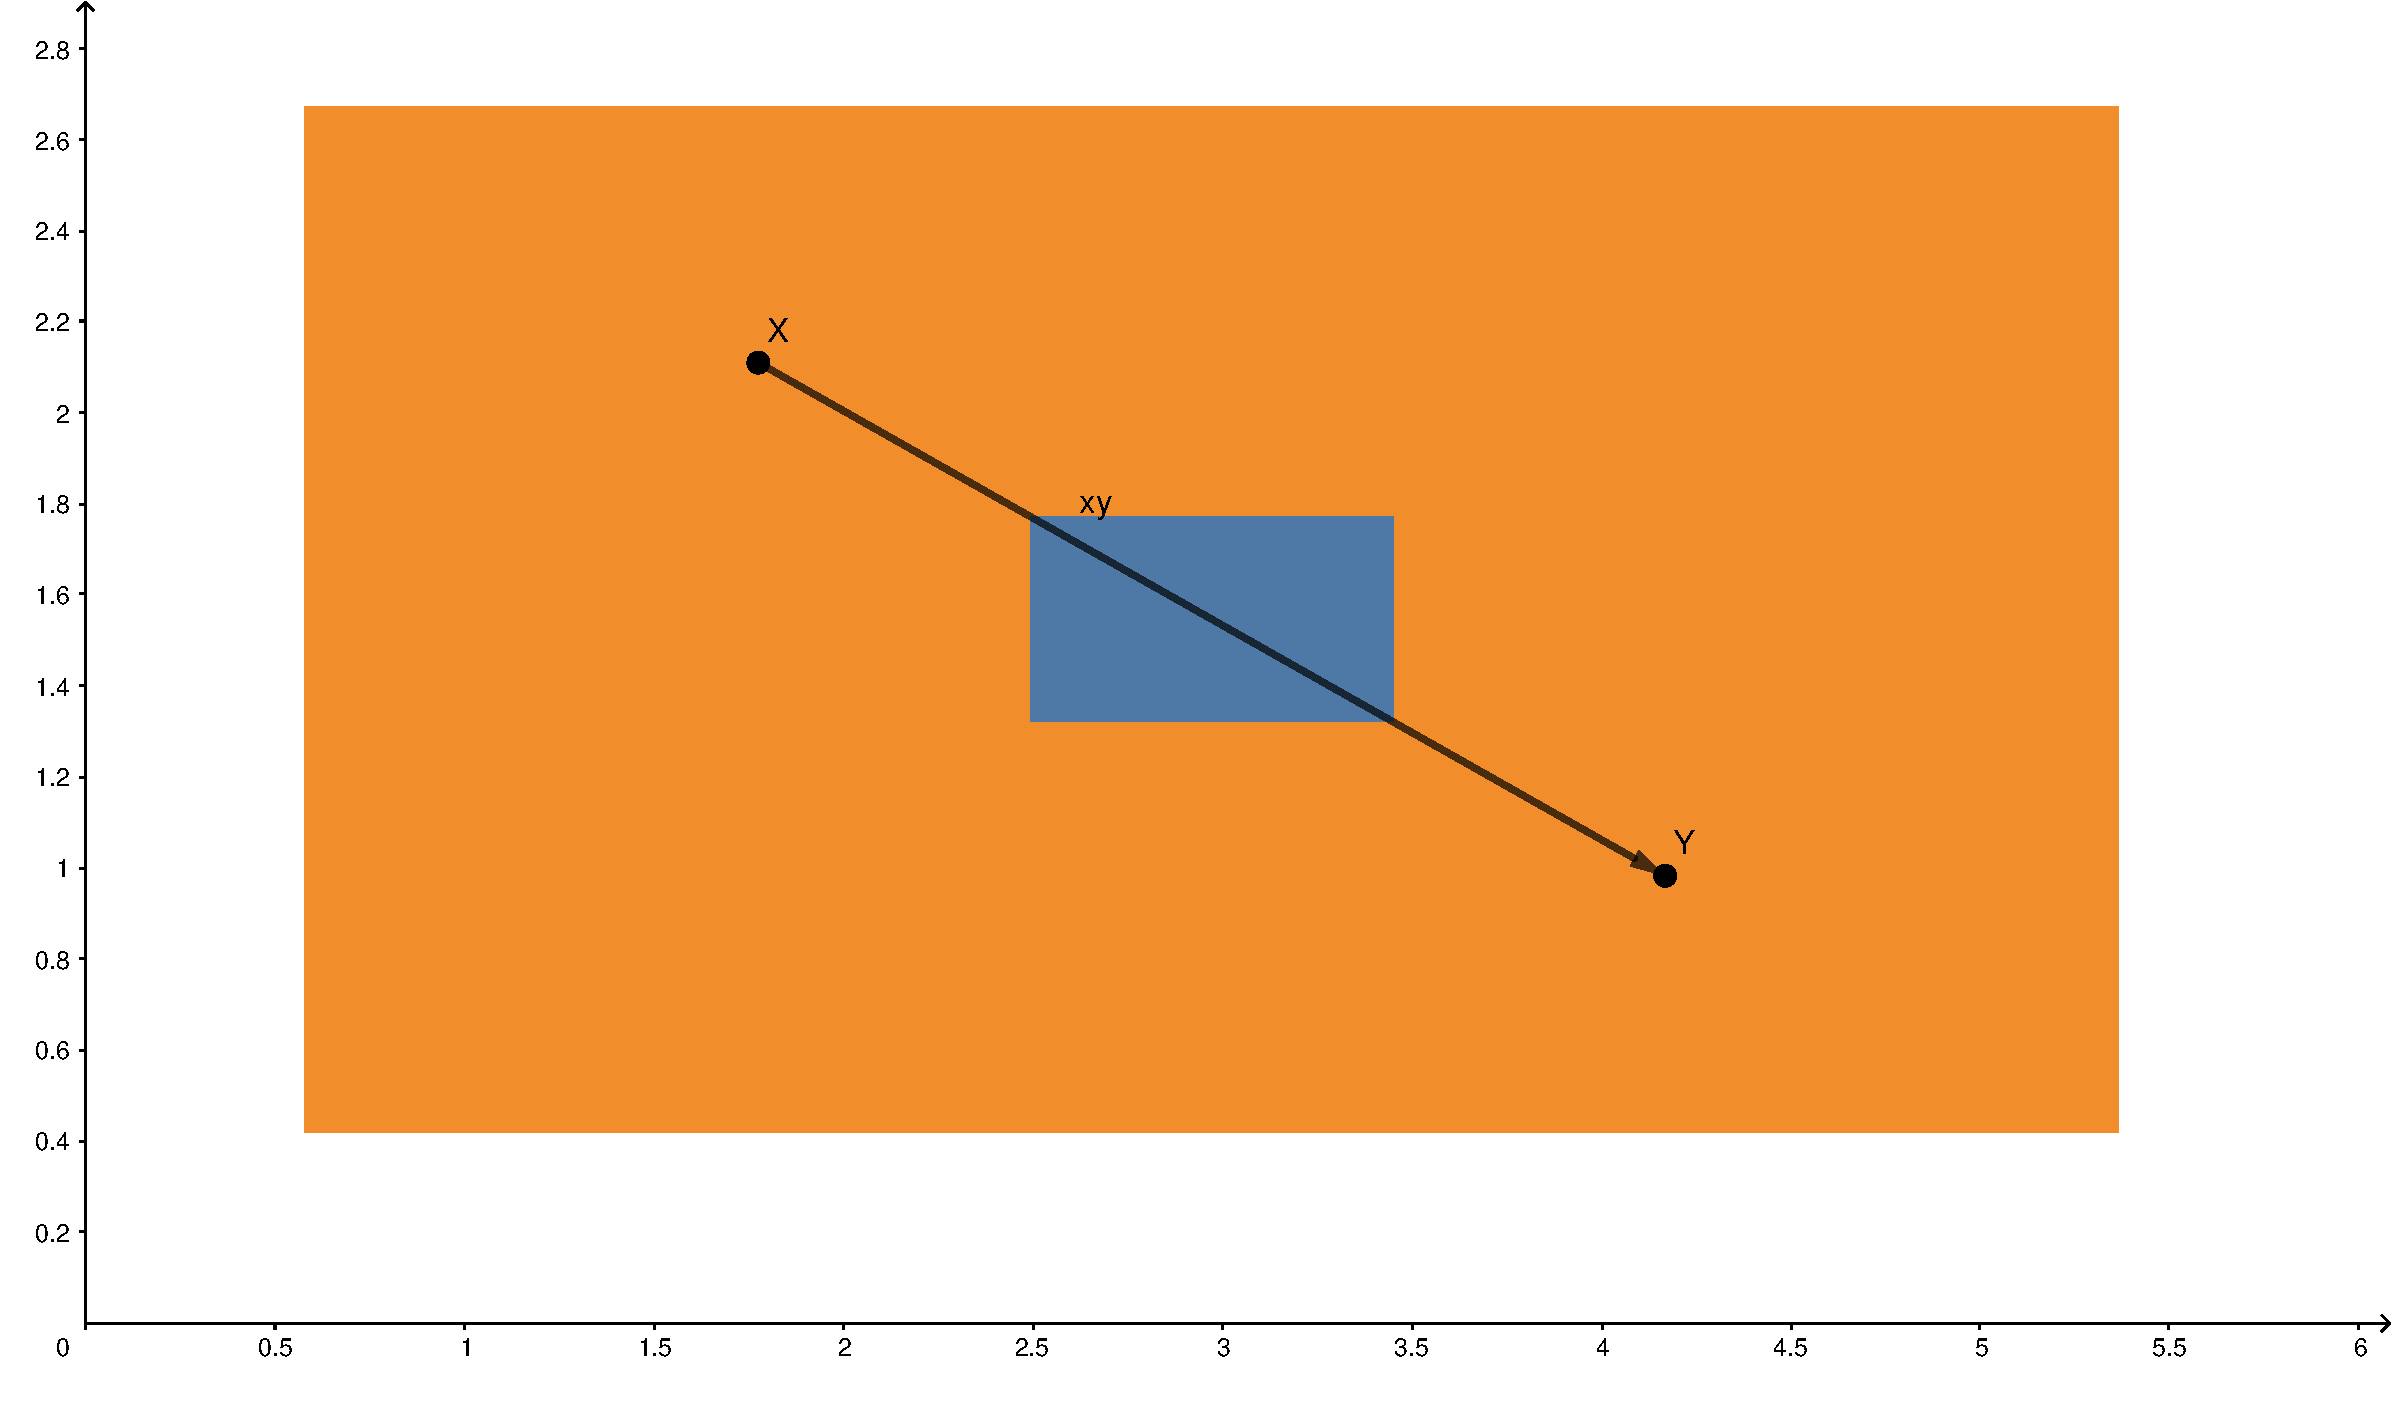
\includegraphics[width=\textwidth]{img/BLX.pdf}
        \caption{Blend crossover sample space with $\alpha=0.5$ (orange) and $\alpha=-0.3$ (blue) in two dimensions.}
        \label{fig:blendcrossoverexample}
    \end{subfigure}
    \hfill
    \begin{subfigure}[t]{0.45\textwidth}
        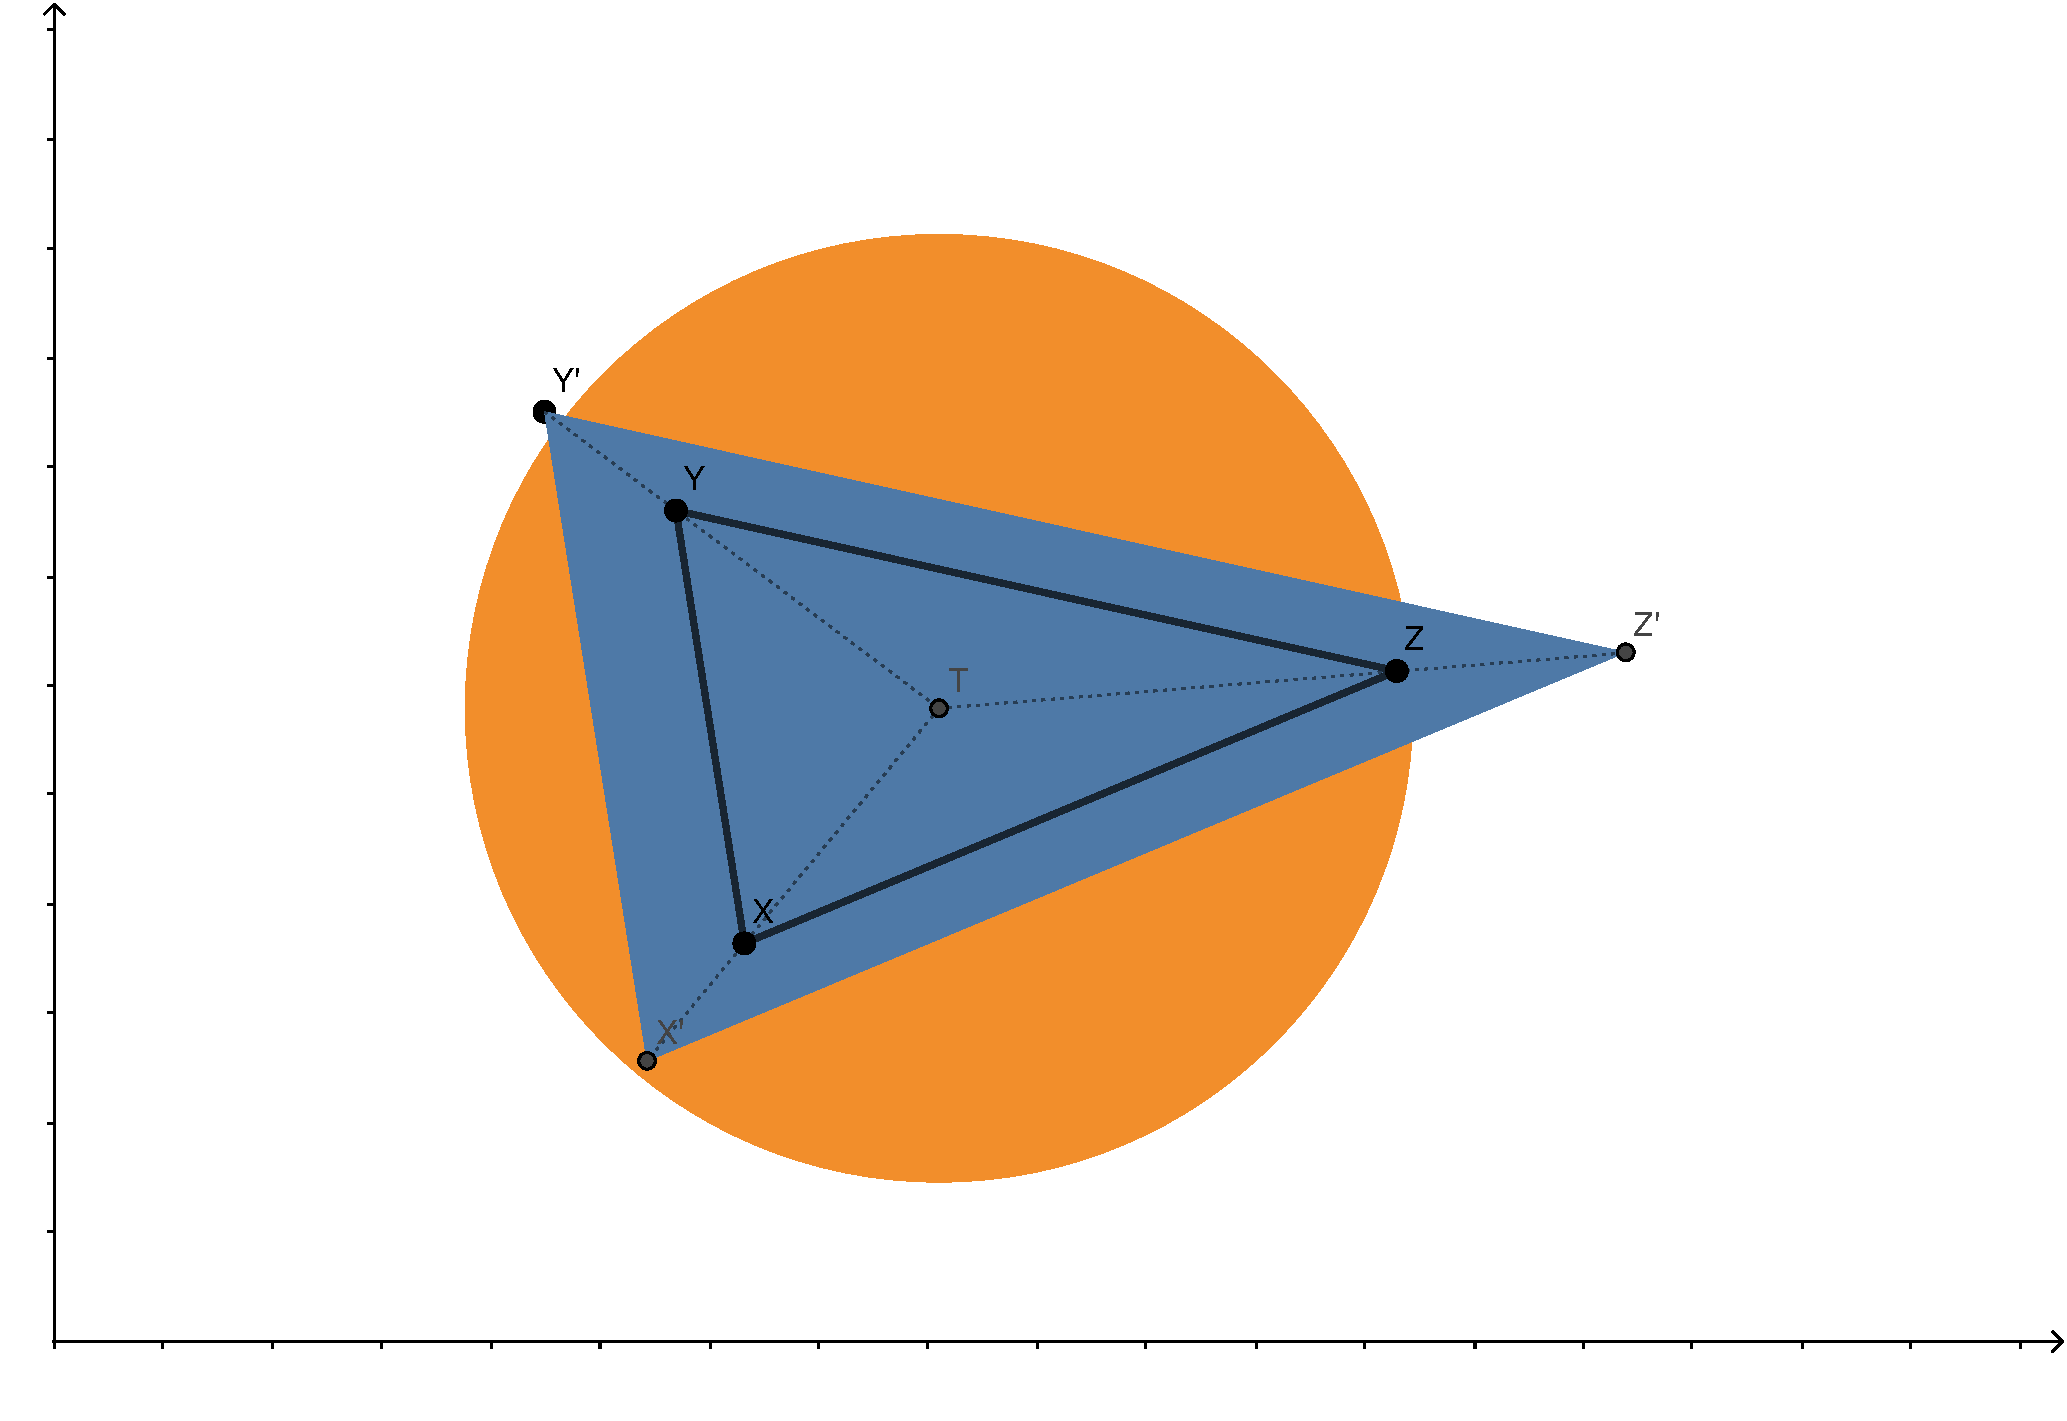
\includegraphics[width=\textwidth]{img/SimplexCrossover.pdf}
        \caption{Simplex crossover example in two dimensions. Sampling space of simplex (blue) and hypersphere (orange).}
        \label{fig:simplexcrossoverexample}
    \end{subfigure}
    \caption{Real--coded crossover operators}
\end{figure}

Another type of crossover operator is \emph{simplex crossover}\index{crossover real--coded!simplex}. It uses simplex to sample sample offsprings. Simplex is a generalization of triangle into more dimensions. It is defined in $n$--dimensional space using $n+1$ points. For two dimensional space is simplex triangle, for three dimensional space is simplex tetrahydron and so on. From the definition, the simplex crossover require $n+1$ parents $\mathbf{p_1}, \mathbf{p_2}, \dots, \mathbf{p_n}, \mathbf{p_{n+1}}$. It calculate their centroid
$$
\mathbf{k}=\frac{\sum_{i=1}^{n+1} \mathbf{p_i}}{n+1}
$$
and then expand the simplex by $\varepsilon$ along each of the direction $\mathbf{p_k} - \mathbf{k}$. As a result, this new, expanded simplex is defined by the points
\boldmath
$$
p'_i = p_i + \varepsilon\left( p_i - k \right).
$$
\unboldmath
From this simplex, the algorithm samples the offspring. Example of simplex in two dimensional space is in the figure \ref{fig:simplexcrossoverexample} with $\varepsilon=1.5$.
I would argue that the hypersphere sample space can be used as well, as is shown in figure \ref{fig:simplexcrossoverexample} as well with $\varepsilon=1.2$.
% TODO not implemented
% In the Introduction to Evolutionary Algorithms, other types of crossovers like Simulated Binary Crossover and Unimodal Normal Distribution Crossover are described as well. I can discuss them when they become relevant.

%%%%%%%%%%%%%%%%%%%%
%%%%  MUTATION  %%%%
%%%%%%%%%%%%%%%%%%%%
\subsection{Real--coded mutation operators}

Equivalent of bit--flip mutation in \acrshort{acc:ga} is \emph{uniform mutation}\index{mutation real--coded!uniform}. It replaces gene by random value sampled from $U(l,u)$ with small probability $p_m$, where interval $\left[l,u\right]$ is the scalar's domain. This operator basically tries random numbers and can rarely lead to a good solution. Moreover, it does not exploit the distribution of the population.

More successful and frequently used is \emph{normal mutation}\index{mutation real--coded!normal}. It performs a little change of the individual by adding sample from a normal distribution with zero mean to each gene.
$$
p_i = p_i + N(0,\sigma)
$$
The $\sigma$ is the mutation strength parameter and is usually kept low. Notice that normal mutation does not use mutation probability $p_m$. Because the $\sigma$ is usually small and the distribution has zero mean, the changes do not influence the population too much.

Normal mutation can be further extended to adapt to more complicated problems. Instead of the $\sigma$ variable, it is possible to introduce $\boldsymbol{\sigma}$ vector, which allows different deviation in each dimension.
$$
p_i = p_i + N(0,\sigma_i)
$$ 
To address non--separable functions, we may need the whole covariance matrix $\Sigma^{n \times n}$ for successful adaptation. Normal mutation with covariance matrix is sometimes called \emph{correlated mutation}. Notice that in order to use correlated mutation in $n$ dimensions, the algorithm needs $\frac{n\left(n+1\right)}{2}$ parameters just for the correlation matrix, and therefore correlated mutation has just a trivial practical usage on its own. Other algorithms address this issue -- probably the \acrfull{acc:cma} is the best--known of them.

The normal distribution is probably the most used mutation distribution, but other distributions are possible as well. \citet*{CauchyDistributionMutation} used Cauchy distribution to faster the search. As shown in figure \ref{fig:mutationdistributionnormalcacuchy}, Cauchy distribution does not decrease as fast as normal distribution and therefore searches more of the genotype space. On the other hand, if we desire to shrink the searching space, we may use polynomial distribution, which probability density function is defined as
$$
p(x)=0.5 \left(n + 1\right)\left( 1 - \abs{x} \right)^n
$$ 
where $n$ user--defined parameter and function domain is interval $\left[-1,1\right]$. Example of polynomial distribution is in figure \ref{fig:mutationdistributionpolynomial}.

\begin{figure}
    \begin{subfigure}[t]{0.45\textwidth}
        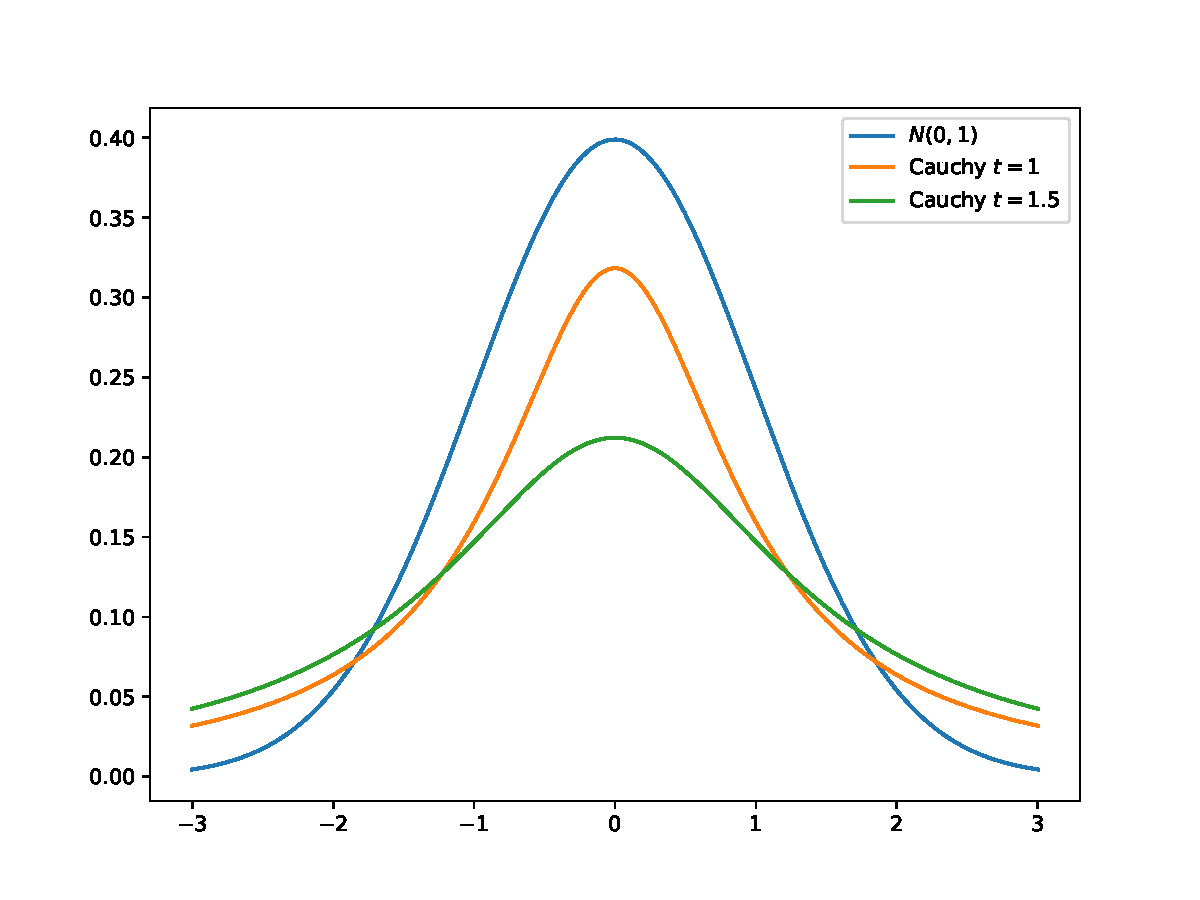
\includegraphics[width=\textwidth]{img/render_distributions_normalcauchy.pdf}
        \caption{Normal and Cauchy distributions}
        \label{fig:mutationdistributionnormalcacuchy}
    \end{subfigure}
    \hfill
    \begin{subfigure}[t]{0.45\textwidth}
        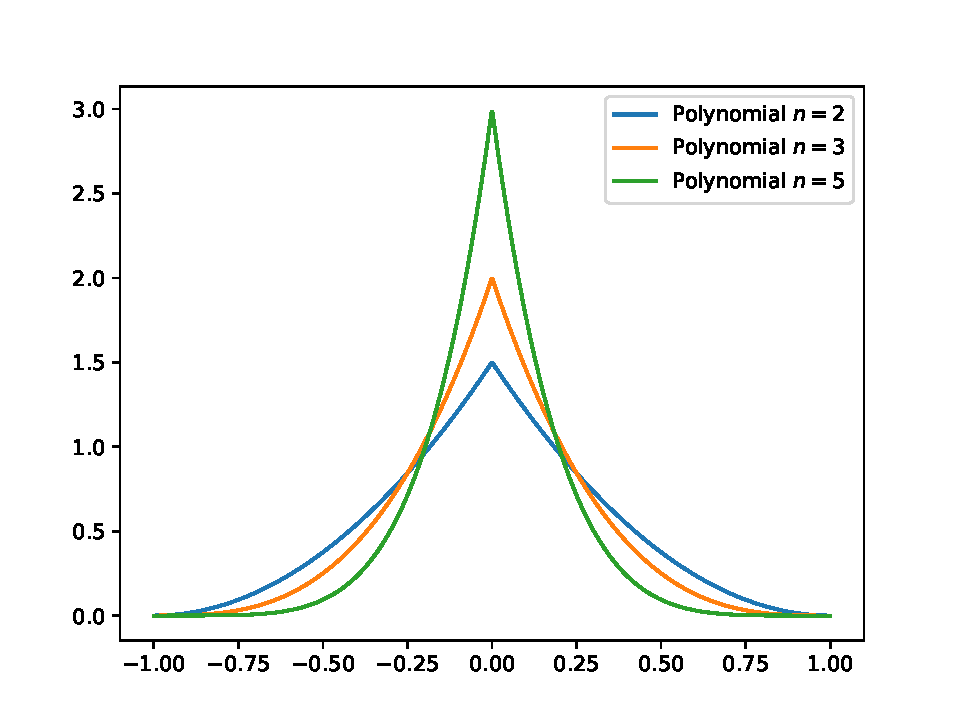
\includegraphics[width=\textwidth]{img/render_distributions_polynomial.pdf}
        \caption{Polynomial distributions}
        \label{fig:mutationdistributionpolynomial}
    \end{subfigure}
    \caption{Mutation distributions}
\end{figure}

%%%%%%%%%%%%%%%%%%%%%%
%%%%  ADAPTATION  %%%%
%%%%%%%%%%%%%%%%%%%%%%
\subsection{Adaptive operators}

It is usually helpful to alter algorithm parameters through evolution to better adjust to the problem at hand. For example, one may decrease the normal distribution deviation in the normal mutation as the population converges to the optimum. \emph{Adaptive operators}\index{adaptive operators} is a general term for operators, which tweak their parameters based on the algorithm's progress.

Decay operators\index{adaptive operators!decay} decrease their value based on the generation number. It may decrease the mutation and crossover probability \citep{DecayGA}, mutation strength, population size, and many more parameters. The central idea behind is that as the algorithm proceeds, the individuals' changes are getting smaller, and the algorithm has a better chance to converge.

One of the most straightforward decay function is linear, that linearly decrease the parameter value from $u$ to $l$.
$$
decay_l(u,l) = u - \frac{g}{G}\cdot\left( u - l \right)
$$
where $g$ is current generation and $G$ is total number of generation. Another popular decay function is exponential:
$$
decay_e(s,r) = s\cdot r^g
$$
where $s$ is starting value of the parameter and $r\in\left[0,1\right]$ is a decay rate. Note that in order to get the same decay rate for a different number of generations, the rate must be reevaluated.
The final decay rate I would like to mention is polynomial decay.
$$
decay_p(s,p) = s \cdot\left(1 - \frac{g}{G}\right)^p
$$
where $s$ is starting value and $p$ is adjustable parameter. Examples of decays are starting at value $5$ and taking $400$ generations are shown in figure \ref{fig:decayrates}.

\begin{figure}
    \centering
    \begin{minipage}[t]{0.48\textwidth}
        \centering
        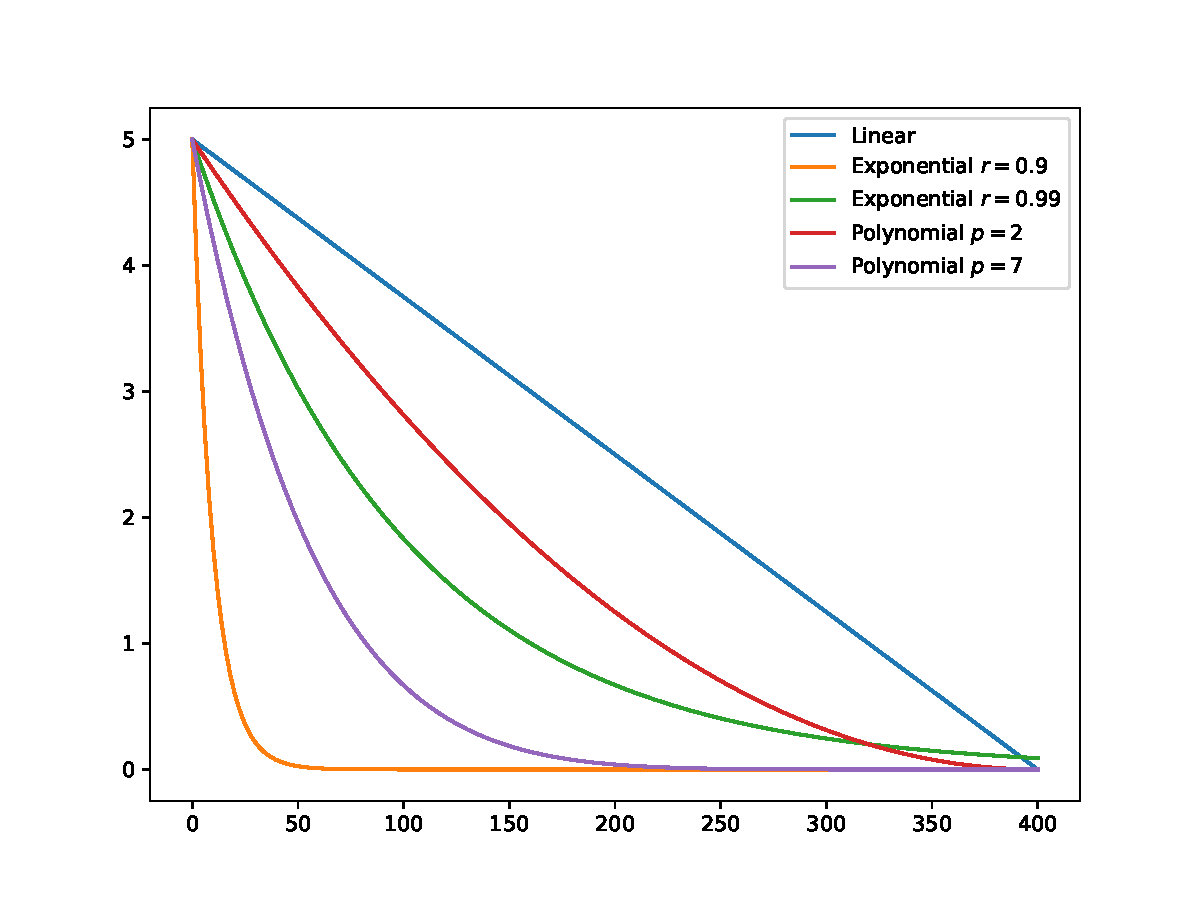
\includegraphics[width=\textwidth]{img/render_decayrate.pdf}
        \caption{Decay rates}
        \label{fig:decayrates}
    \end{minipage}
    \hfill
    \begin{minipage}[t]{0.48\textwidth}
        \centering
        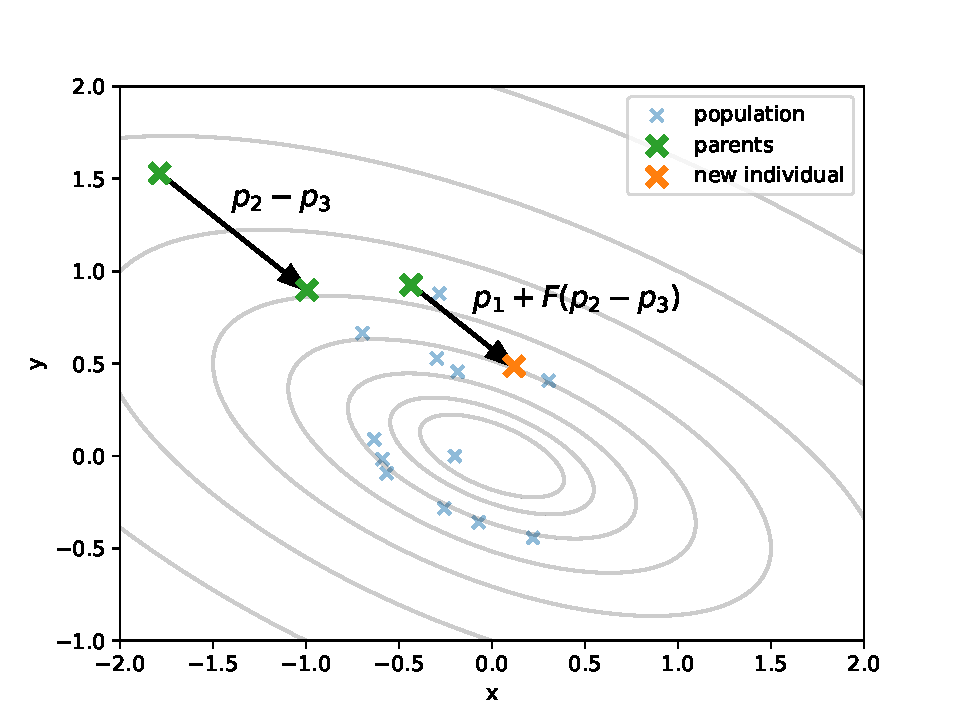
\includegraphics[width=\textwidth]{img/render_differential.pdf}
        \caption[Differential evolution crossover]{Differential evolution crossover with $F=0.7$}
        \label{fig:differentialevolution}
    \end{minipage}
\end{figure}

Another popular approach to adaptive operators is the \emph{one--fifth rule}\index{adaptive operators!one--fifth rule} \citep{onefifthrule}. The main idea behind is to increase mutation deviation (usually called step--size) after successful mutation and decrease it otherwise. The reasoning behind this is that if too many individuals are better, then the search is probably too local, and by increasing the step size, we increase the search domain. Consequently, a few successful individuals indicate that the step is too big and should decrease.

As a rule, authors \citet*{onefifthruleoriginal} suggested $1/5$ success rate as the threshold value. If at least $1.5$ offsprings are better, then the step--size should be increased by a factor of $1.5$ and decreased by a factor of $1.5^{-1/4}$ otherwise \citep{onefifthrule}.

However, the proof of this rule by \citeauthor*{onefifthruleoriginal} was done only for unimodal function and small populations. It is generally not a good balance for more complex problems. Better results can be achieved using more advanced techniques to adapt parameters, such as \acrshort{acc:cma}.

%%%%%%%%%%%%%%%%%%%%%%%%%%%%%%%%%%
%%%%  DIFFERENTIAL EVOLUTION  %%%%
%%%%%%%%%%%%%%%%%%%%%%%%%%%%%%%%%%
\subsection{\texorpdfstring{\acrlong*{acc:de}}{Differential evolution}}

\acrfull{acc:de}\index{differential evolution} is a kind of real--coded evolutionary algorithm, suggested by \citet*{differentialevolutionoriginal}. \acrshort{acc:de} apply special operation to the population, that combines crossover, mutation, and selection. \acrshort{acc:de} is sometimes considered as a directional--based search technique, because it takes into account distribution of the individuals in the population. It can therefore manage non--separable functions better in comparison to traditional real--coded evolutionary algorithms.

\acrshort{acc:de} uses four distinct parents $\mathbf{p_1}, \mathbf{p_2}, \mathbf{p_3}, \mathbf{p_4}$. It first construct trial vector $v$ such that
$$
\mathbf{v} = \mathbf{p_1} + F\left( \mathbf{p_2} - \mathbf{p_3} \right)
$$
where $F$ is user--defined positive parameter controlling the strength of the direction. The vector $\mathbf{p_2} - \mathbf{p_3}$ is the direction from parent $\mathbf{p_3}$ to parent $\mathbf{p_2}$ and reflects the correlation within the population. One example is in the figure \ref{fig:differentialevolution}. Notice how a newly created individual is much closer to the optimum compared to its parents.

There is a possibility to use more parents and combine them. Moreover, there are possibilities not to sample parents uniformly but substitute the best individual in the population as either $\mathbf{p_1}$ or $\mathbf{p_2}$. Alternatively, it is possible to use the same individual as the source of the direction, as well as the starting position.Mathematically  express by substitution $\mathbf{p_1} = \mathbf{p_3}$. The formula for the crossover with five parents is
$$
\mathbf{v} = \mathbf{p_1} + F_1\left( \mathbf{p_2} - \mathbf{p_3} \right) + F_2\left( \mathbf{p_4} - \mathbf{p_5} \right)
$$

Last but not least, this crossover operator can be easily used within traditional real--coded evolutionary algorithms as well.

After the crossover, \acrshort{acc:de} performs uniform crossover between the trial vector $\mathbf{v}$ and parent $\mathbf{p_4}$ to finally create offspring $\mathbf{o}$. The mutation rate is controlled by a parameter $C\in\left[0,1\right]$ that represent a probability of offspring $\mathbf{o}$ inherits gene from trial vector $\mathbf{v}$. Finally, the offspring $\mathbf{o}$ is compared to the original parent $\mathbf{p_4}$ and replace it, if is better. This step is equivalent of selection and \acrshort{acc:de} is kind of steady--state evolution strategy, as defined on page \pageref{enum:steadystate}.




%%%%%%%%%%%%%%%%%%%%%%%%%%%%%%%%%%%
%%                               %%
%%  Particle swarm optimization  %%
%%                               %%
%%%%%%%%%%%%%%%%%%%%%%%%%%%%%%%%%%%
\section{\texorpdfstring{\acrlong*{acc:pso}}{Particle swarm optimization}}

\acrfull{acc:pso}\index{particle swarm optimization} is another population--based stochastic optimization technique inspired by a flocking of birds and schooling of fish in Nature. It was introduced by \citet*{PSOOriginal}. The \acrshort{acc:pso} is somehow similar to the real--coded evolutionary algorithms and \acrshort{acc:es} in the sense that the individual is a vector of real numbers. In the \acrshort{acc:pso} terminology, the individuals are called \emph{particles}.

Thorough the time, the \acrshort{acc:pso} went through plenty of improvements. Two major versions, namely \acrfull{acc:spso2006} and \acrfull{acc:spso2011}, were released as a baseline for further improvements. I will focus on these versions as specified by \citet{SPSO}.

Except for the position, each particle $\mathbf{p_i}$ has velocity vector $\mathbf{v_i}$, which defines the particle's direction and speed. The velocity vector is then used for a position update. Unlike real--coded evolutionary algorithms, modifications to the particles are not made directly but by manipulating with the velocity vector. These two components are the cause why the \acrshort{acc:pso} get its name.

Additionally to velocity, each particle $\mathbf{p_i}$ remember it's own best position, usually called \emph{local best}\index{particle swarm optimization!local best} and denoted by $\mathbf{L_i}$. This variable is updated after every step if the particle's fitness value is better than the fitness value of $\mathbf{L_i}$.

Similarly, each particle remembers the best position it received from the swarm, usually called \emph{global best}\index{particle swarm optimization!global best} and denoted by $\mathbf{G_i}$. After each step, each particle informs surrounding particles about its position and fitness value. Each particle may inform a different set of particles. Which particles to inform is defined by particle's \emph{neighborhood}, and I will focus on it a bit later. Each particle then accumulates information from its surrounding and may update its global best position $\mathbf{G_i}$.

\begin{algorithm}
    \KwIn{$s$ population size, $steps$ number of steps, $\fitnessfn$ fitness function}
    \ForEach{particle $i$ in $1$..$s$}{
        Initialize particle position $\mathbf{p_i}$\;
        Initialize particle velocity $\mathbf{v_i}$\;
        Initialize local and best positions $\mathbf{L_i}=\mathbf{G_i}=\mathbf{p_i}$\;
    }
    \ForEach{$step$ in $0$..$steps$}{
        \ForEach{particle $i$ in $1$..$s$}{
            Update velocity $\mathbf{v_i}$ based on $\mathbf{p_i}$, $\mathbf{L_i}$, and $\mathbf{G_i}$\;
            Update position $\mathbf{p_i}$ based on $\mathbf{v_i}$\;
            \If{$\fitnessfn(\mathbf{p_i})$ is better than $\fitnessfn(\mathbf{L_i})$}{
                $\mathbf{L_i}\leftarrow\mathbf{p_i}$\;
            }
            \ForEach{particle $j$ in $Neighborhood(i)$}{
                \If{$\fitnessfn(\mathbf{p_i})$ is better than $\fitnessfn(\mathbf{G_j})$}{
                    $\mathbf{G_j}\leftarrow\mathbf{p_i}$\;
                }
            }
        }
    }
    \Return{particle $\mathbf{p_k}$ such that $k = \argmin\limits_{i}\fitnessfn(\mathbf{p_i})$}
    \caption{General \acrfull*{acc:pso} algorithm}
    \label{alg:PSOgeneral}
\end{algorithm}

The algorithm of general \acrshort{acc:pso} algorithm is in algorithm \ref{alg:PSOgeneral}. The difference between \acrshort{acc:spso2006} and \acrshort{acc:spso2011} is in the way they update the velocity $\mathbf{v_i}$.

%%%%%%%%%%%%%%%%%%%%%%%%
%%%%  NEIGHBORHOOD  %%%%
%%%%%%%%%%%%%%%%%%%%%%%%
\subsection{Neighborhood}

Neighborhood\index{particle swarm optimization!neighborhood} or also called topology, specifies connections between particles and how the particles communicate their best positions in the swarm. It directly controls information flow in the swarm and therefore speed of convergence. For a big neighborhood, the particles soon receive the best position in the swarm and will attempt to reach it without much exploring. If the neighborhood is too small, particles may focus too much on the exploration as the global information would be missing.

\begin{figure}[t]
    \begin{subfigure}[t]{0.3\textwidth}
        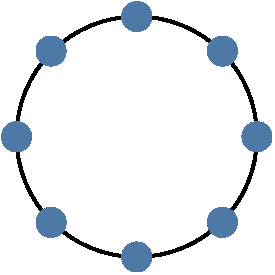
\includegraphics[width=\textwidth]{img/master_neigh_ring.pdf}
        \caption{Ring topology}
        \label{fig:topologyring}
    \end{subfigure}
    \hfill
    \begin{subfigure}[t]{0.3\textwidth}
        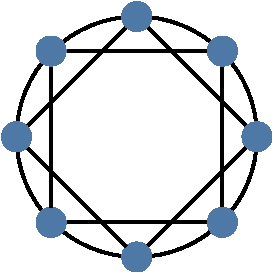
\includegraphics[width=\textwidth]{img/master_neigh_densering.pdf}
        \caption{Dense ring topology}
        \label{fig:topologydensering}
    \end{subfigure}
    \hfill
    \begin{subfigure}[t]{0.3\textwidth}
        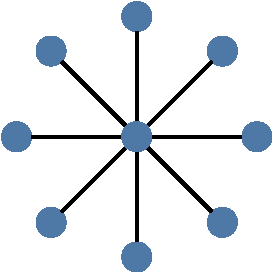
\includegraphics[width=\textwidth]{img/master_neigh_star.pdf}
        \caption{Star topology}
        \label{fig:topologystar}
    \end{subfigure}
    \caption{\acrshort*{acc:pso} neighborhood topologies}
\end{figure}

Some of the popular neighborhood topologies are ring (figure \ref{fig:topologyring}), dense ring (figure \ref{fig:topologydensering}), and star (figure \ref{fig:topologystar}). Moreover, particles can be organized in the grid and allow communication only within this grid. Some popular grid topologies are linear (figure \ref{fig:topologygridlinear}), diamond (figure \ref{fig:topologygriddiamond}), and compact (figure \ref{fig:topologygridcompact}) \citep{PSOtopologies}.

\begin{figure}[b]
    \begin{subfigure}[t]{0.3\textwidth}
        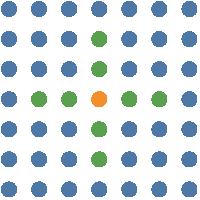
\includegraphics[width=\textwidth]{img/master_neigh_linear.pdf}
        \caption{Linear grid topology}
        \label{fig:topologygridlinear}
    \end{subfigure}
    \hfill
    \begin{subfigure}[t]{0.3\textwidth}
        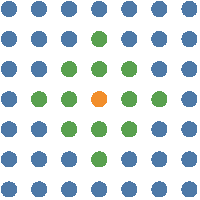
\includegraphics[width=\textwidth]{img/master_neigh_diamond.pdf}
        \caption{Diamond grid topology}
        \label{fig:topologygriddiamond}
    \end{subfigure}
    \hfill
    \begin{subfigure}[t]{0.3\textwidth}
        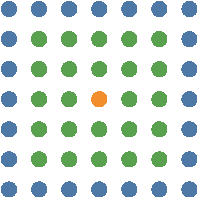
\includegraphics[width=\textwidth]{img/master_neigh_compact.pdf}
        \caption{Compact grid topology}
        \label{fig:topologygridcompact}
    \end{subfigure}
    \caption[\acrshort*{acc:pso} grid topologies]{\acrshort*{acc:pso} grid topologies. Population is colored blue, active particle orange and it's neighborhood by green.s}
\end{figure}

Notice that all these topologies are static and do not change during the run of the algorithm. Dynamic topologies were proposed, such as random topology and closest neighbors topology. In the random topology, each particle informs $k$ random particles from the swarm. The $k$ is usually kept small, for example $k=3$ \citep{SPSObenchmark}. Note that different neighborhood is generated after each step. In the closest neighbors topology, each particle informs $k$ closest particles -- except that this topology is very computation--intensive, it usually leads to premature convergence because particles begin to create clusters and keep informing themselves only within this cluster. On the other hand, it has prerequisites to find multiple local minima in a single run.

%%%%%%%%%%%%%%%%%%%%
%%%%  VELOCITY  %%%%
%%%%%%%%%%%%%%%%%%%%
\subsection{Velocity update}

Difference between \acrshort{acc:spso2006} and \acrshort{acc:spso2011} is the way they change velocity. In \acrshort{acc:spso2006}, the velocity update is
$$
\mathbf{v_i} = \omega\mathbf{v_i} 
+ c_l U_d\left( 0,1 \right) \cdot \left( \mathbf{L_i} - \mathbf{p_i} \right)
+ c_g U_d\left( 0,1 \right) \cdot \left( \mathbf{G_i} - \mathbf{p_i} \right)
$$ 
where $\omega$ is inertia weight, $c_l$ and $c_g$ are cognitive respectively social acceleration coefficients, and $U_d(0,1)$ is independent and uniformly distributed random vector in the range $\left[ 0,1 \right]$ with dimension $d$. The $\cdot$ is an element--wise multiplication. The inertia weight prevents the explosion of the velocity. Constants $c_l$ and $c_g$ controls how much the local best respectively the global best attracts the particle and are specified by the user. The particle position is then updated simply by adding applying velocity to the particle.
$$
\mathbf{p_i} = \mathbf{p_i} + \mathbf{v_i}
$$

Except for inertia weight, one may limit the particle's position to fit into the interval of interest, respectively, limit velocity. We may limit the velocity using its magnitude (then no particle can move faster than a specified threshold) or per coordinate, similarly to the position \citep{PSOvelocitylimit}.

\begin{figure}
    \begin{subfigure}[t]{0.45\textwidth}
        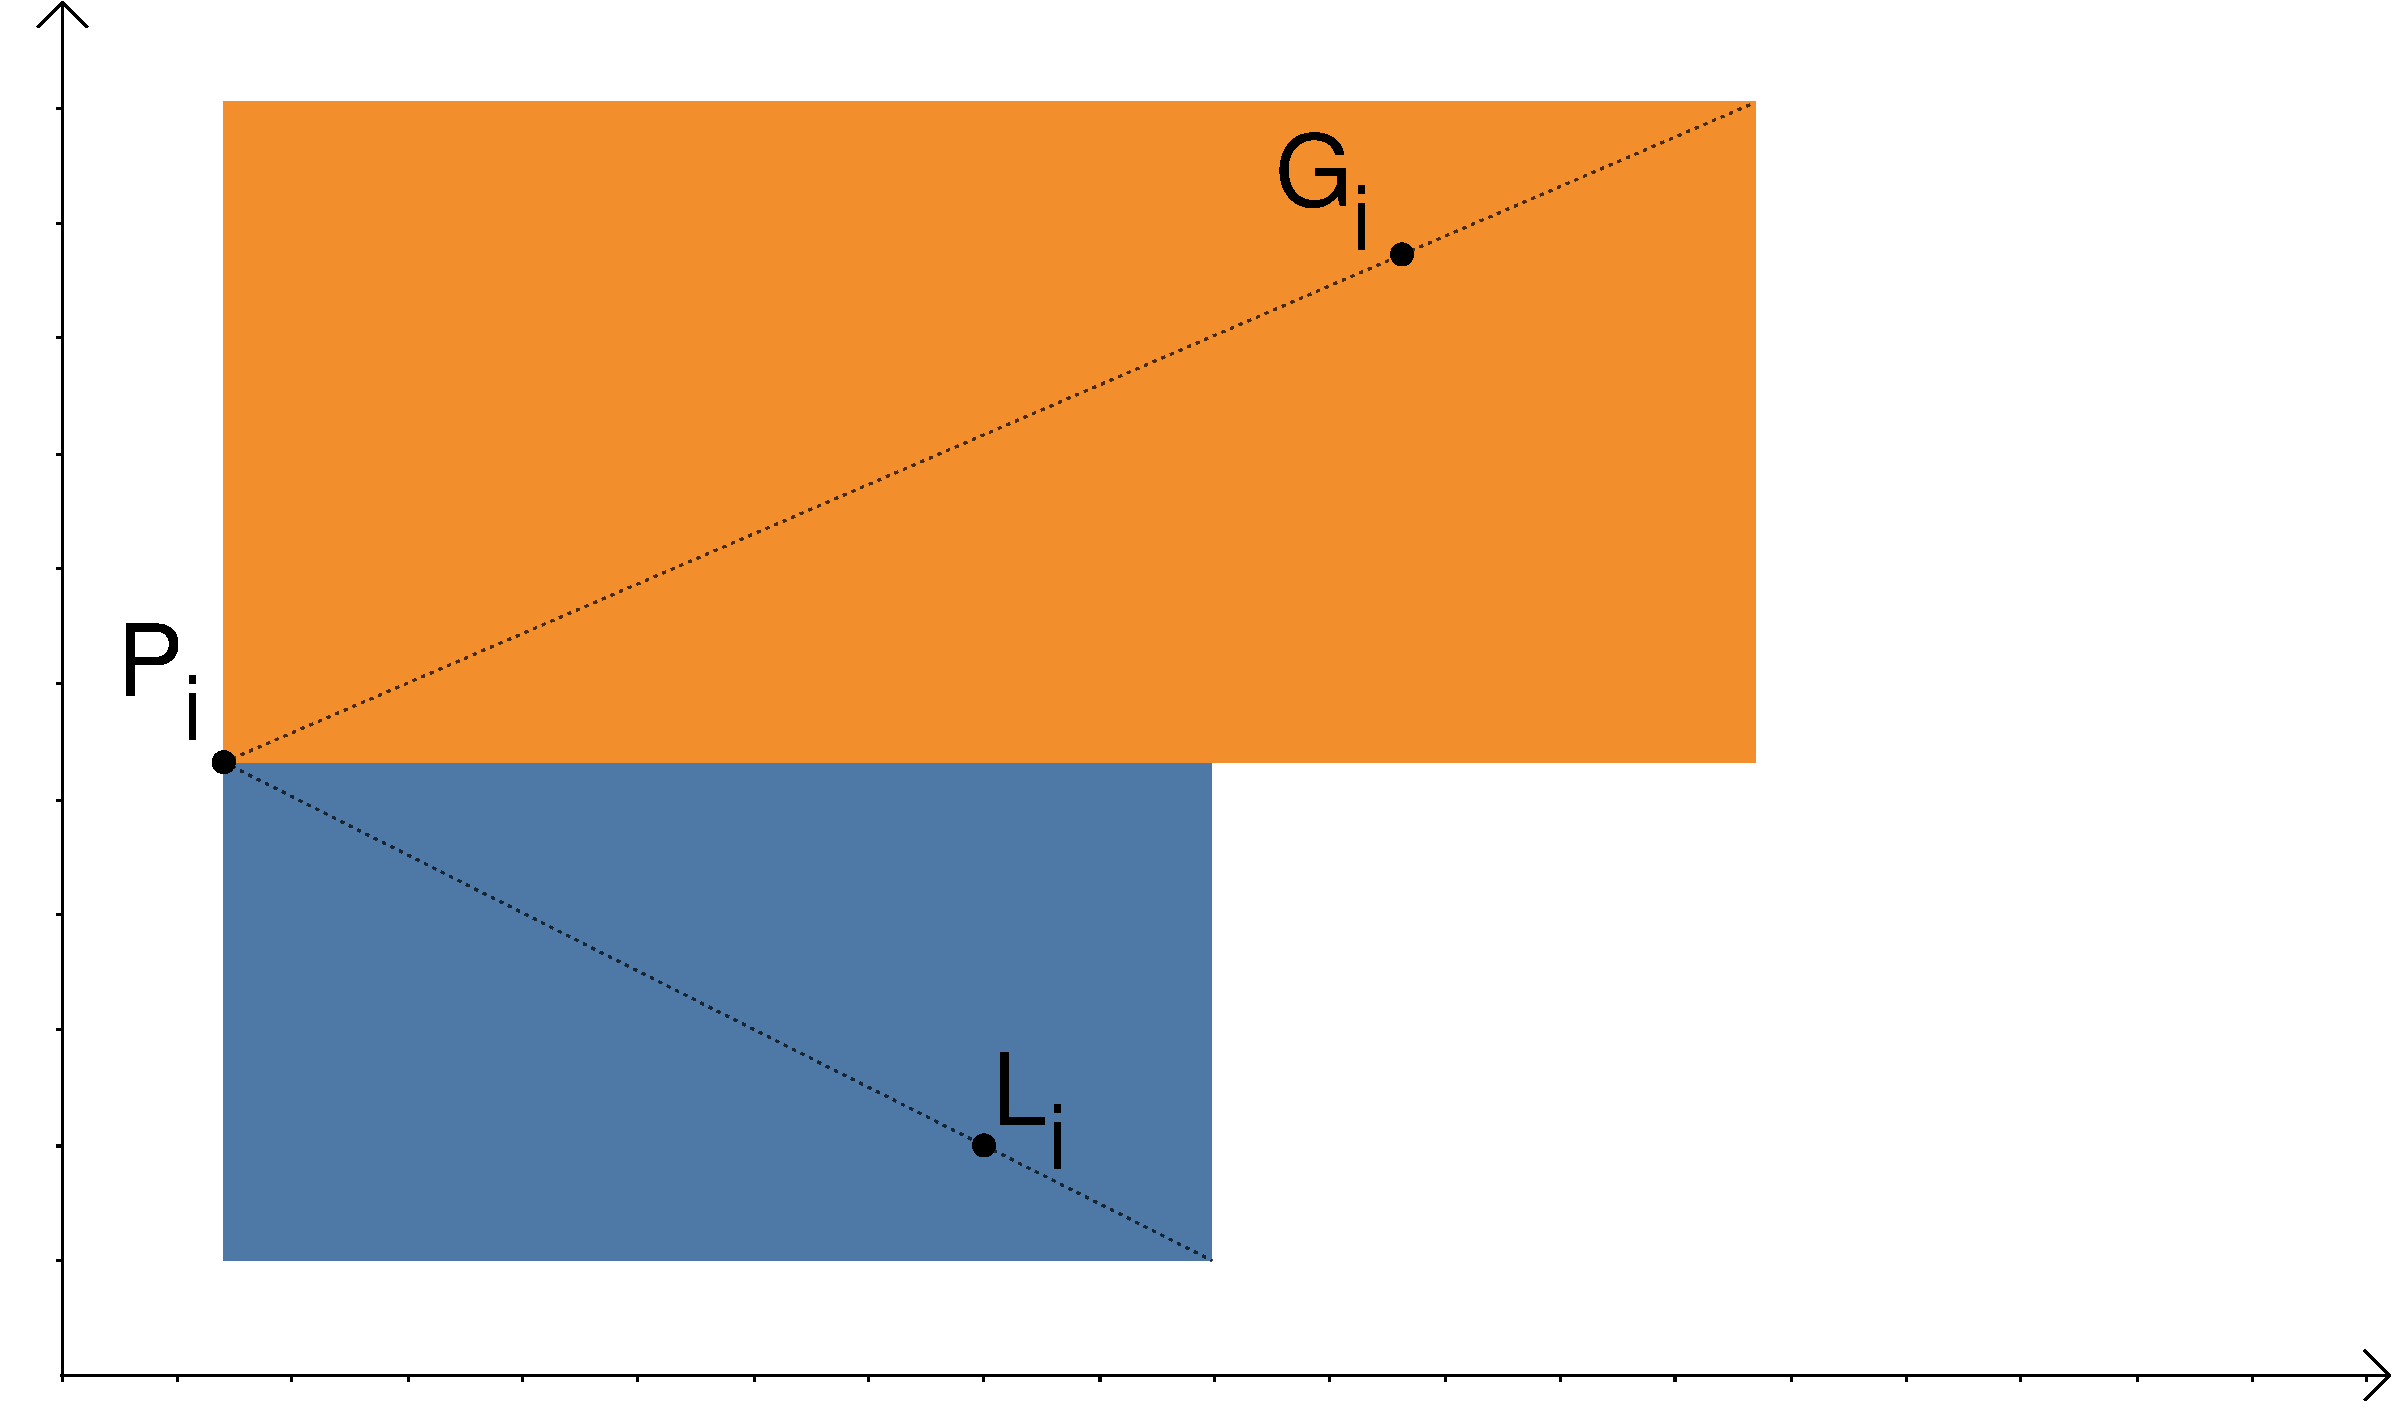
\includegraphics[width=\textwidth]{img/pso2006.pdf}
        \caption{\acrshort*{acc:spso2006} sampling space}
        \label{fig:samplingspso2006}
    \end{subfigure}
    \hfill
    \begin{subfigure}[t]{0.45\textwidth}
        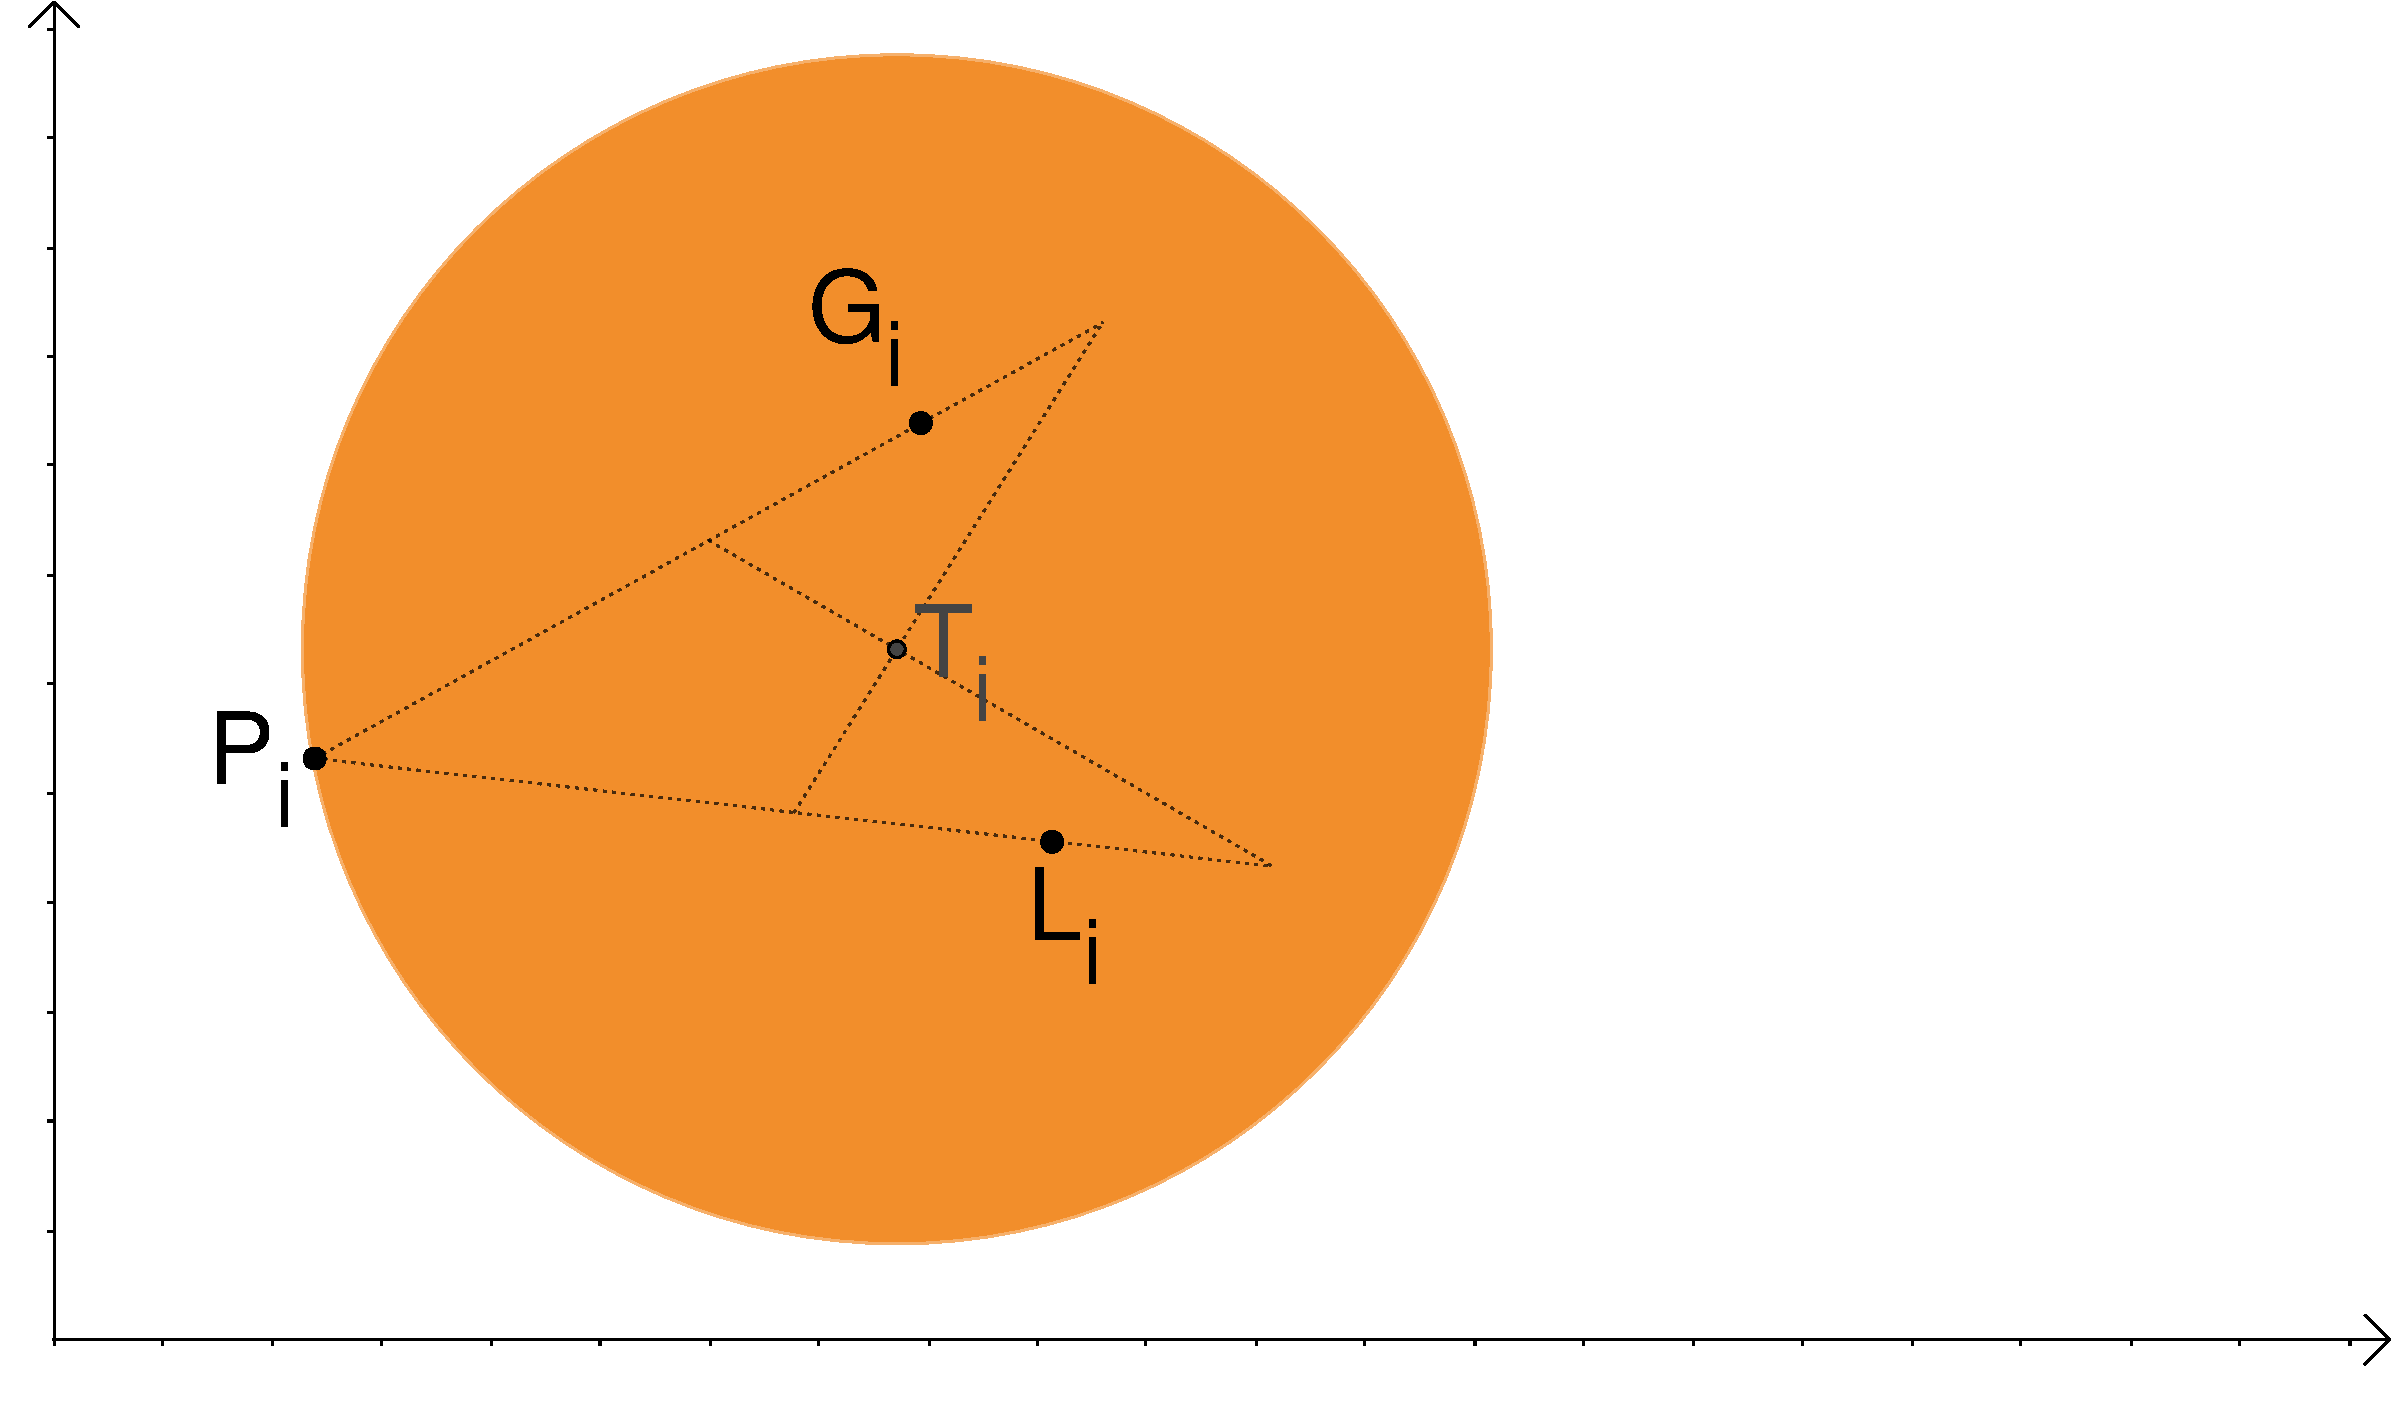
\includegraphics[width=\textwidth]{img/pso2011.pdf}
        \caption{\acrshort*{acc:spso2011} sampling space}
        \label{fig:samplingspso2011}
    \end{subfigure}
    \caption{Sampling space of \acrshort*{acc:spso2006} and \acrshort*{acc:spso2011}}
\end{figure}

Because the velocity update in \acrshort{acc:spso2006} is done dimension by dimension, the algorithm's performance is rotation sensitive and coordinate system dependent. This phenomenon is visible in figure \ref{fig:samplingspso2006}. The sampled point for the local respectively global best position is sampled from the blue respectively orange region. As these regions align with axes, the resulting sampling is aligned with axes as well. It has been shown \citep{psobiasinzero} that it is easier for \acrshort{acc:spso2006} to find optimum if it lies in the center of coordinate systems or on the axis.

\acrshort{acc:spso2011} address this issue by sampling the point from hypersphere. First of all, it finds center of gravity $\mathbf{T}$ between current, local best, and global best positions.
\begin{align*}
    \mathbf{l_i} &= \mathbf{p_i} + c_l U_d\left( 0,1 \right) \cdot \left( \mathbf{L_i} - \mathbf{p_i} \right) \\
    \mathbf{g_i} &= \mathbf{p_i} + c_g U_d\left( 0,1 \right) \cdot \left( \mathbf{G_i} - \mathbf{p_i} \right) \\
    \mathbf{T_i} &= \frac{\mathbf{p_i}+\mathbf{l_i}+\mathbf{g_i}}{3}
\end{align*}
Random point is then sampled from the hypersphere with the center $\mathbf{T_i}$ and radius $\norm{\mathbf{P_i} - \mathbf{T_i}}$
$$
\mathbf{u_i} = \mathcal{H}_i\left(\mathbf{T_i}, \norm{\mathbf{P_i} - \mathbf{T_i}}\right)
$$
Velocity update then simply adds direction to this point to the previous velocity.
$$
\mathbf{v_i} = \omega\mathbf{v_i}+\mathbf{u_i}-\mathbf{p_i}
$$
The sample space for two dimensions is shown in figure \ref{fig:samplingspso2011}.
